\chapter{Data-driven background estimation}\label{chap:bkgmodel}

\section{Motivation}
An extrapolation procedure was chosen due to the broad deviations in the gradient of the mass spectrum resulting from non-resonant signatures. A fit over the full invariant mass spectrum would bais the background estimation as the background only fit would attempt to accommodate the broad deviations at high-mass. It has been shown previously by the dilepton resonance search~\cite{Aad:2019fac} and diphoton searches~\cite{Aaboud:2016tru,Aaboud:2017yyg} that similar background shapes to the one in this search can be modelled with a suitable function. The fits are constrained at the low-mass regions, where there is an abundance of statistics to provide a rigid background description. Therefore, the background model is fit in a low mass control region (CR), and the resulting fit is extrapolated to a high mass signal region (SR). An illustration of the extrapolation procedure outlining the CR and SR is shown in \cref{fig:bkgmodel:ranges}.

There are several challenges involved with the extrapolation approach. One challenge is the choice of function picked to model the fit in the low-mass control region and the high mass extrapolation. A central part of the analysis is quantifying the bias introduced by choice of a particular function and quantifying the uncertainty on both the shape and normalisation of the extrapolated background. An optimisation procedure is performed in two consecutive steps. The first involves the choice of the fit function. An initial sample of roughly 25 functions are validated in a set of potential CR and SR region configurations. Once the function is fixed, the CR and SRs are optimised using the function to maximise sensitivity and reduce the bias of the background estimation. The choice of function, CR and SR, and estimation of uncertainties are described in the sections below. All fits are performed within the RooFit~\cite{RooFit} framework.

\begin{figure}[!htpb]
    \centering
    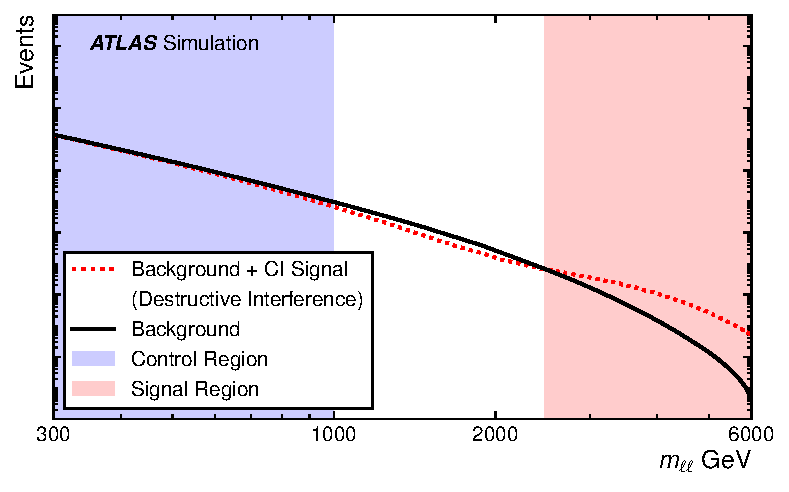
\includegraphics[width=0.8\textwidth]{/Users/Deshan/Documents/PhD/thesis/Thesis/figures/analysis/bkgmodel/fig_01a.pdf} 
    \caption[A schematic illustration of the possible mass ranges in this analysis.]{A schematic illustration of the possible mass ranges in this analysis.
    The monotonically falling total background shape is shown by the solid black line, while an example of a CI signal plus the total background shape is shown by the dotted red line. The CI signal is shown after the DY process has been subtracted to show only the interference and pure CI process. The gap illustrated between the CR and the SR is found to be the preferred case for the destructive interference cases only.}
    \label{fig:bkgmodel:ranges}
\end{figure}

\section{Background function choice}\label{sec:modelchoice}
The functional form used to fit the background is chosen from a variety of different candidates for its stability during the extrapolation procedure, and the ability to model the invariant mass distributions of the \ee and \mumu channels. Each function is fit to the background dilepton invariant mass template, produced by summing together the contributions from all the background processes, in a variety of different CRs and extrapolated to the corresponding SRs. The distribution of the pulls, defined as (fit-simulation)/fit, is obtained for each invariant mass bin for all initial CR and SR ranges considered. Functions which have pulls below 2 in the CR and SRs are marked as acceptable. This requirement ensures that functions which exhibit unphysical behaviour in the tails of the invariant mass spectrum are vetoed. Additionally, it ensures that good modelling of the simulated shape in the CR is maintained. There were a possible three functions which satisfied the above conditions. Regardless of the choice of final function, each function that satisfies the initial selection criteria will have inherent weaknesses in their bias and performance. These are then measured and taken into account as uncertainties, described in \cref{sec:extrap:uncertainties}. The final function was chosen out of the subset of functions to be consistent with the sister analysis~\cite{Aad:2019fac}. The fit function is given in \cref{eq:fitfunc}. 
\begin{equation}
    \label{eq:fitfunc}
    \begin{aligned}
        & f_\textrm{b}(m_{\ell\ell}) = f_{\mathrm{BW},Z}(m_{\ell\ell}) \cdot \left(1 - x^{c}\right)^{b} \cdot x^{\sum_{i=0}^3 p_i\log(x)^i}, \\
        & f_{\mathrm{BW},Z}(\mathrm{m_{\ell\ell}}) = \frac{\Gamma_Z}{(m_Z - \mathrm{m_{\ell\ell}})^2 + \Gamma_Z^2},
    \end{aligned}
\end{equation}

where $x = m_{\ell\ell}/\sqrt{s}$. The first term, $f_{\mathrm{BW},Z}(m_{\ell\ell})$, is a non-relativistic Breit--Wigner function with $m_Z = \SI{91.1876}{\giga\electronvolt}$ and $\Gamma_Z = \SI{2.4952}{\giga\electronvolt}$~\cite{PhysRevD.98.030001}. The $(1 - x^{c})$ ensures that the background fit evaluates to zero as $x \to 1$, to be consistent with the expectation from the collision energy of the LHC. Both b and c are chosen to be fixed based on fits to the full background template. The $p_i$ parameters, with $i = 0,..,3$, are left as free parameters to be informed by the fit. 

The fits to the data and simulation are both performed with a bin width of \SI{1}{\giga\electronvolt}. The function $f_b(m_{\ell\ell})$ is treated as a probability density in the fits performed to the CR. It is normalised in the CR to the number of events in the CR ($N_{CR}$) of the template being fit. \cref{fig:bkgmodel:fitstoMC} shows an example of background only fits to the electron and muon channel in a CR and SR configuration. The binning of the plots were changed to be constant in $\log{(\text{m}_{\ell\ell})}$ from 230--\SI{6000}{\giga\electronvolt} for f presentation, as figures with the linear \SI{1}{\giga\electronvolt} binning will be difficult to interpret clearly. In \cref{fig:fitstoMC2} some disagreement between in the fit and the and the background template can be seen in the SR a high mass. However, the difference corresponding number of events between the extrapolation and background template will be very small in the single-bin SR.

\begin{figure}[h!]
    \centering
    \begin{subfigure}[b]{0.49\textwidth}
        \centering
        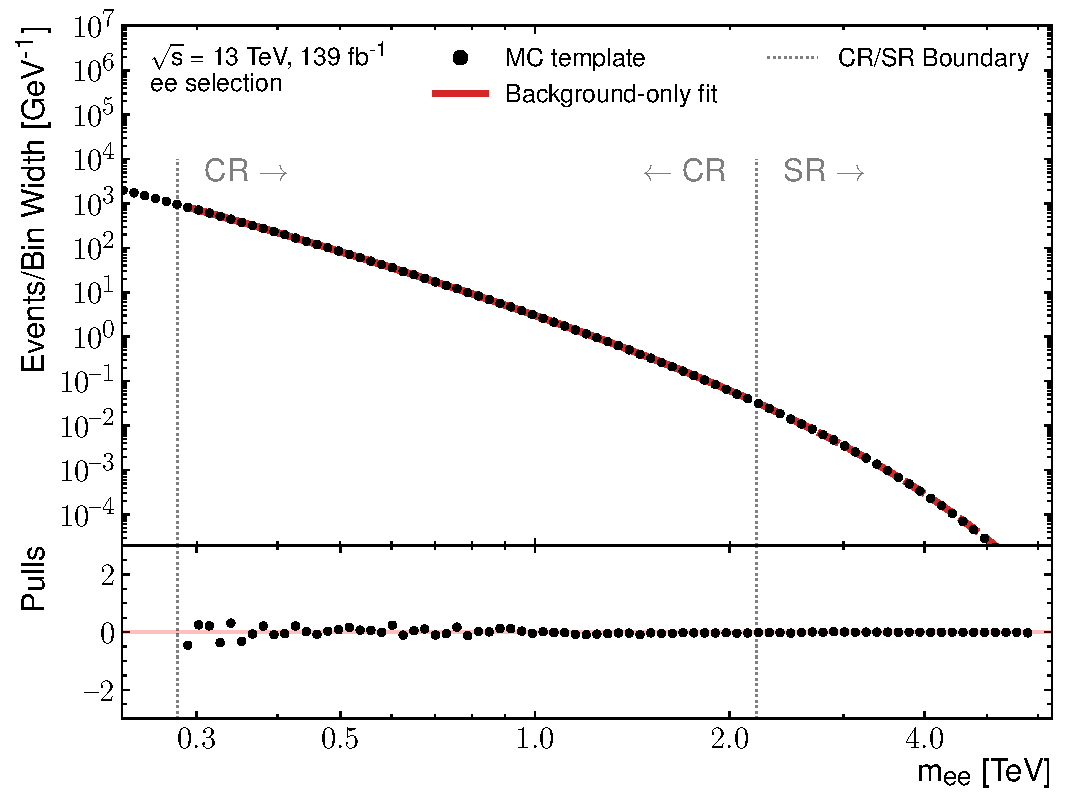
\includegraphics[width=\textwidth]{/Users/Deshan/Documents/PhD/thesis/Thesis/figures/analysis/bkgmodel/fit-const-ee-backgroundModel.pdf}
        \label{fig:fitstoMC1}
    \end{subfigure}
    \begin{subfigure}[b]{0.49\textwidth}
        \centering
        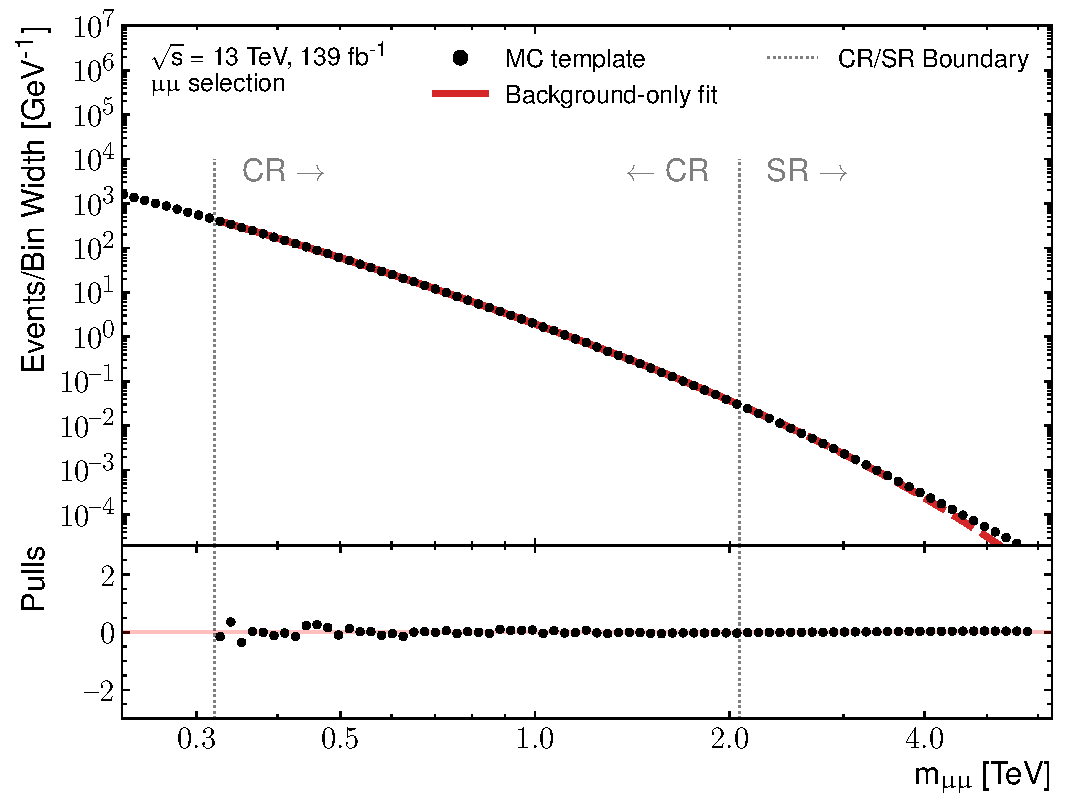
\includegraphics[width=\textwidth]{/Users/Deshan/Documents/PhD/thesis/Thesis/figures/analysis/bkgmodel/fit-const-mm-backgroundModel.pdf}
        \label{fig:fitstoMC2}
    \end{subfigure}
    \caption[Fits to the simulated background template in the electron and muon channels]{fit to the simulated background template in the electron (left) and muon (right) channels shown in the top pad. The bottom pad shows the pulls of the fit. The CR and SR boundaries are also shown in the figure. The background template points are plotted at the centre of each bin as the number of events divided by the bin width, which is constant in $\log{(\text{m}_{\ell\ell})}$.}
    \label{fig:bkgmodel:fitstoMC}
\end{figure}

Examples of functions that did not satisfy the above criteria are given in \cref{tab:bkgmodel:functions}, with their corresponding fits to the data shown in \cref{fig:bkgmodel:badfitstomc}. Nonphysical behaviour in the fit and  extrapolation can be seen in \cref{fig:bkgmodel:fitstoMC5}. \cref{fig:bkgmodel:fitstoMC4,fig:bkgmodel:fitstoMC6} were not selected due to poor modelling of the CR. \cref{fig:bkgmodel:fitstoMC3} depicts a function fit that is close to satisfying the function choice selection. However, it poorly models the extrapolated region compared to the function defined in \cref{eq:fitfunc}.

\begin{table}[h!]
    \centering
    \begin{tabular}{c|l}
         & Function definition \\
        \hline\hline 
        1 & $(1 - x^{5})^{\text{p0}}*(x^{(\text{p1} + \text{p2}*\log(x)})$ \\
        2 & $(1-\log(e*x^{\text{p1}})+c1*x*e^{\text{p2}/(1+x^{\text{p3}})}$ \\
        3 & $(x)^{\text{p1}}*e^{\text{p2}*x}$\\
        4 & $(1-x)^{\text{p1}}*e^{\text{p2}*x^2}$ \\
	\end{tabular}
    \caption[List of functions considered for the background fit]{List of functions considered for fit to dilepton spectrum that did not pass the criteria required. $x$ is defined to be $= m_{\ell\ell}/\sqrt{s}$. }
    \label{tab:bkgmodel:functions}
\end{table}

\begin{figure}[h!]
    \centering
    \begin{subfigure}[b]{0.49\textwidth}
        \centering
        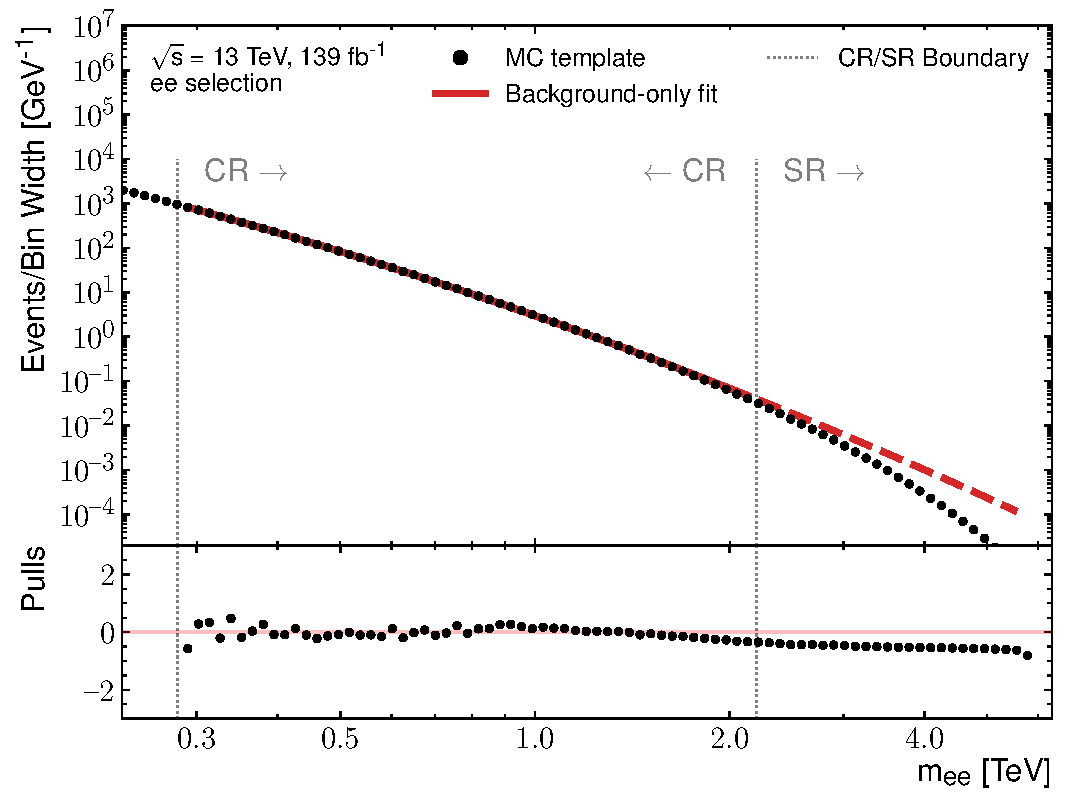
\includegraphics[width=\textwidth]{/Users/Deshan/Documents/PhD/thesis/Thesis/figures/analysis/bkgmodel/fit-const-ee-diphoton3.pdf}
        \caption{}
        \label{fig:bkgmodel:fitstoMC3}
    \end{subfigure}
    \begin{subfigure}[b]{0.49\textwidth}
        \centering
        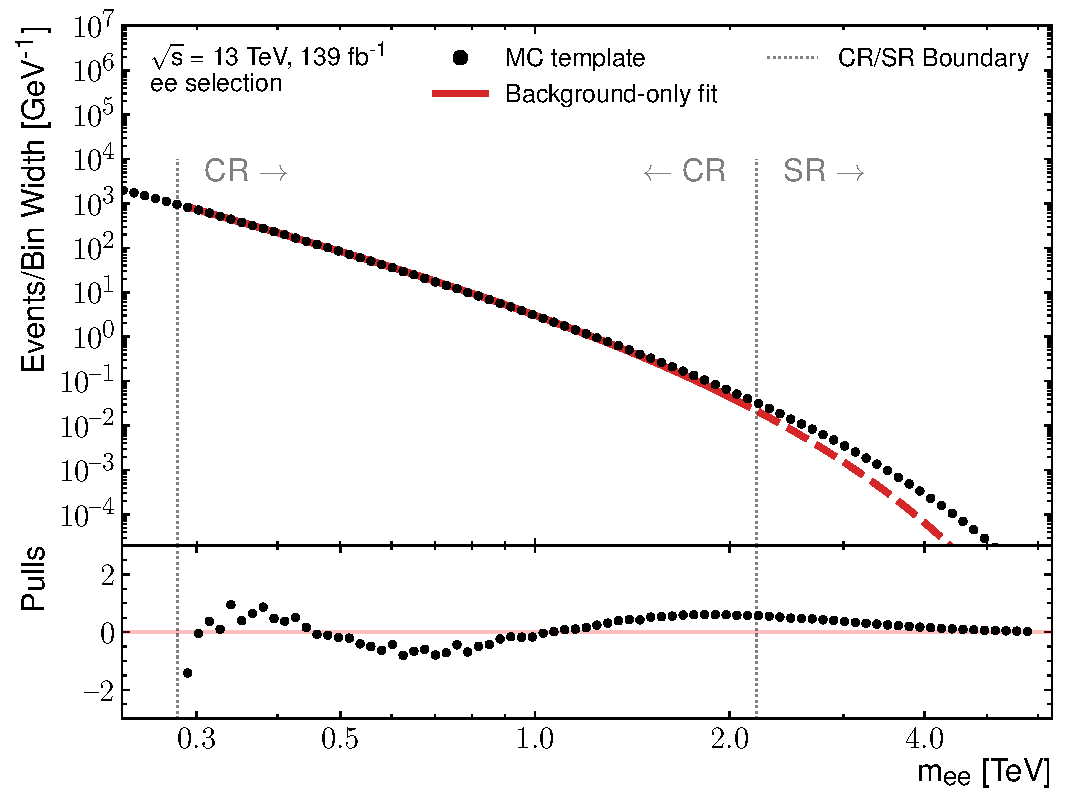
\includegraphics[width=\textwidth]{/Users/Deshan/Documents/PhD/thesis/Thesis/figures/analysis/bkgmodel/fit-const-ee-dext1.pdf}
        \caption{}
        \label{fig:bkgmodel:fitstoMC4}
    \end{subfigure}
    \begin{subfigure}[b]{0.49\textwidth}
        \centering
        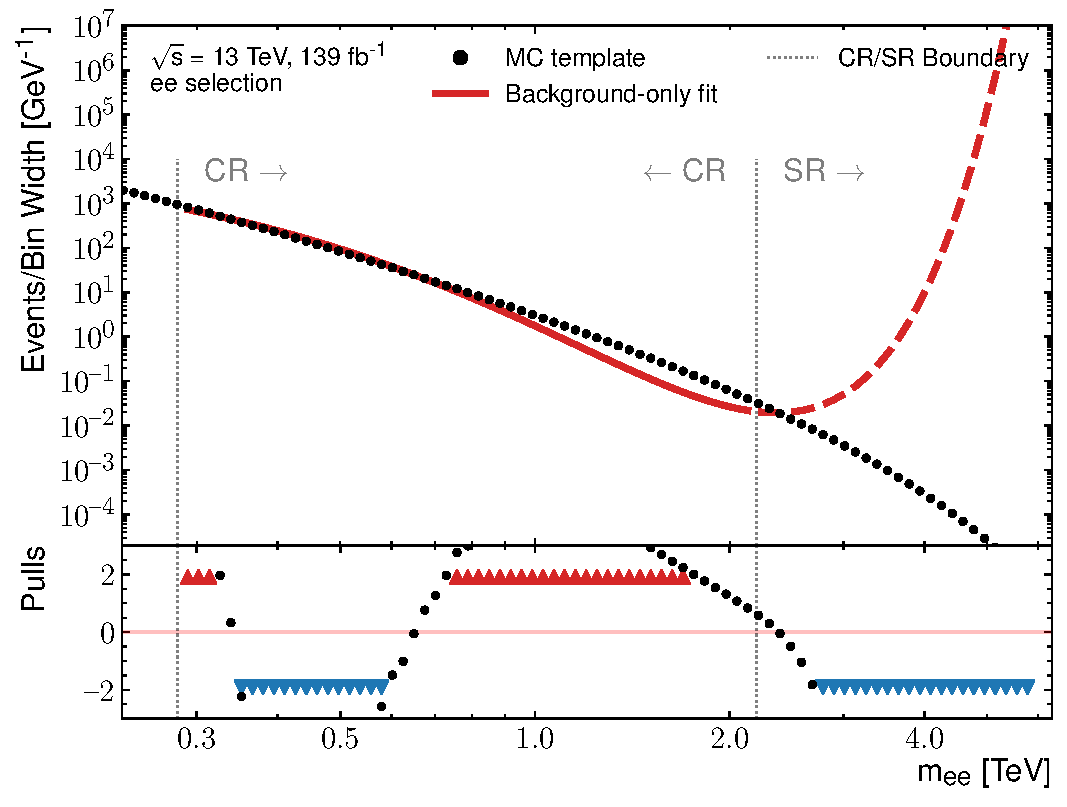
\includegraphics[width=\textwidth]{/Users/Deshan/Documents/PhD/thesis/Thesis/figures/analysis/bkgmodel/fit-const-ee-multijetf2.pdf}
        \caption{}
        \label{fig:bkgmodel:fitstoMC5}
    \end{subfigure}
    \begin{subfigure}[b]{0.49\textwidth}
        \centering
        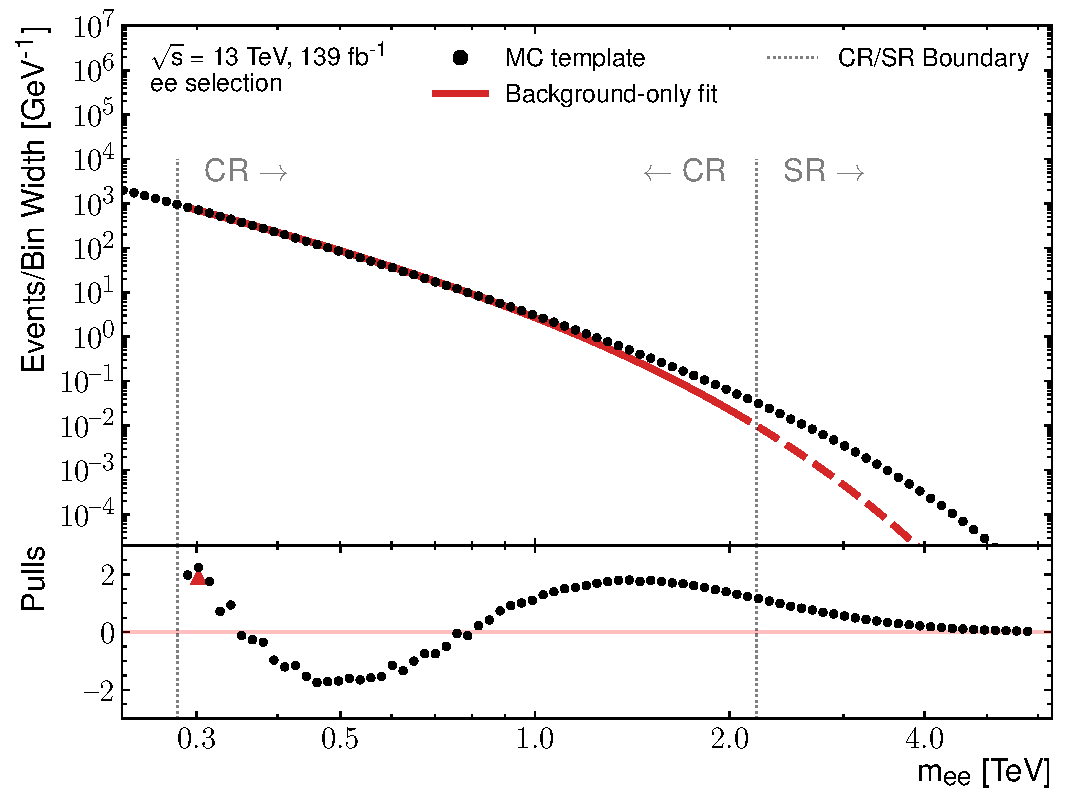
\includegraphics[width=\textwidth]{/Users/Deshan/Documents/PhD/thesis/Thesis/figures/analysis/bkgmodel/fit-const-ee-UA2_1.pdf}
        \caption{}
        \label{fig:bkgmodel:fitstoMC6}
    \end{subfigure}
    \caption[Fits to the simulated background template in the electron and muon channels using functions that did not pass the selection criteria]{Fits using functions that failed the function choice criteria, to the simulated background template in the electron channel shown in the top pad. Figures (a), (b), (c) and (d) correspond to functions 1, 2, 3, and 4 in \cref{tab:bkgmodel:functions}, respectively. The bottom pad shows the pulls of the fit. The CR and SR boundaries are also shown in the figure. The background template points are plotted at the centre of each bin as the number of events divided by the bin width, which is constant in $\log{(\text{m}_{\ell\ell})}$.}
    \label{fig:bkgmodel:badfitstomc}
\end{figure}
\clearpage

\section{Signal model}\label{sec:sigmodel}
The CR region choice is validated using a signal+background model in order to avoid bias from possible signal contamination in the CR. Signal injection tests are performed in each of the CR and SR region configurations. A collection of signal samples at various $\Lambda$ values are injected into the background template, and the effect on the background estimation from the fit and extrapolation is checked. The signal+background fit model is formed by adding a signal component is added to \cref{eq:fitfunc}: 
\begin{equation}
    \label{eq:sbfunction}
    \begin{aligned}
    f_\textrm{b+s}(m_{\ell\ell},\Lambda) = N_\textrm{b}\cdot f_\textrm{b}(m_{\ell\ell}) + N_\textrm{s}(\Lambda)\cdot f_\textrm{s}(m_{\ell\ell},\Lambda),
    \end{aligned} 
\end{equation}
where $f_\textrm{s}(m_{\ell\ell},\Lambda)$ is the signal probability density function and $N_\textrm{s}(\Lambda)$ is the number of signal events in the CR. Both $f_\textrm{s}(m_{\ell\ell},\Lambda)$ and $N_\textrm{s}(\Lambda)$ are determined from simulation. The morphing procedure, described in \cref{sec:datamc:mc:sig:morphing} is used to obtain a smooth descriptions of a given CI model as function of $\Lambda$, allowing to determine signal contributions that fall between the fixed signal shapes from simulation. The parameter $N_\textrm{b}$ is the number of background events in the CR with the constraint $N_\textrm{b}+N_\textrm{s}(\Lambda)=N_\textrm{CR}$. 

\cref{fig:bkgmodel:sbfits} depicts signal+background fits to a background template injected with a CI interaction signal at $\Lambda = \SI{26}{\tera\electronvolt}$ in the electron and muon channels. The background component of the signal+background fit is separated and compared with the background template, and the pulls are calculated. The figure shows that the background component of the signal+background fit is not biased by the presence of a signal in the control region. 
\begin{figure}[h!]
    \centering
    \begin{subfigure}[b]{0.49\textwidth}
        \centering
        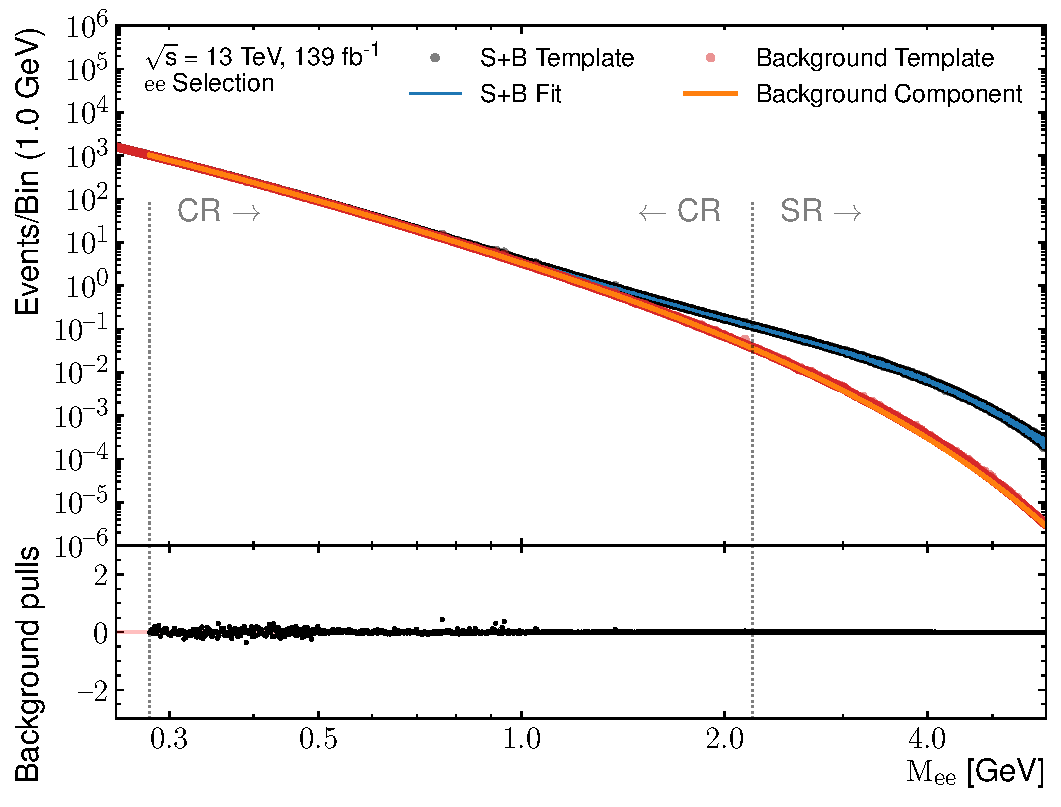
\includegraphics[width=\textwidth]{/Users/Deshan/Documents/PhD/thesis/Thesis/figures/analysis/bkgmodel/nominalFit-sb-const-LL-18-sbTrue-ee-.pdf}
        \label{fig:bkgmodel:sbfits1}
    \end{subfigure}
    \begin{subfigure}[b]{0.49\textwidth}
        \centering
        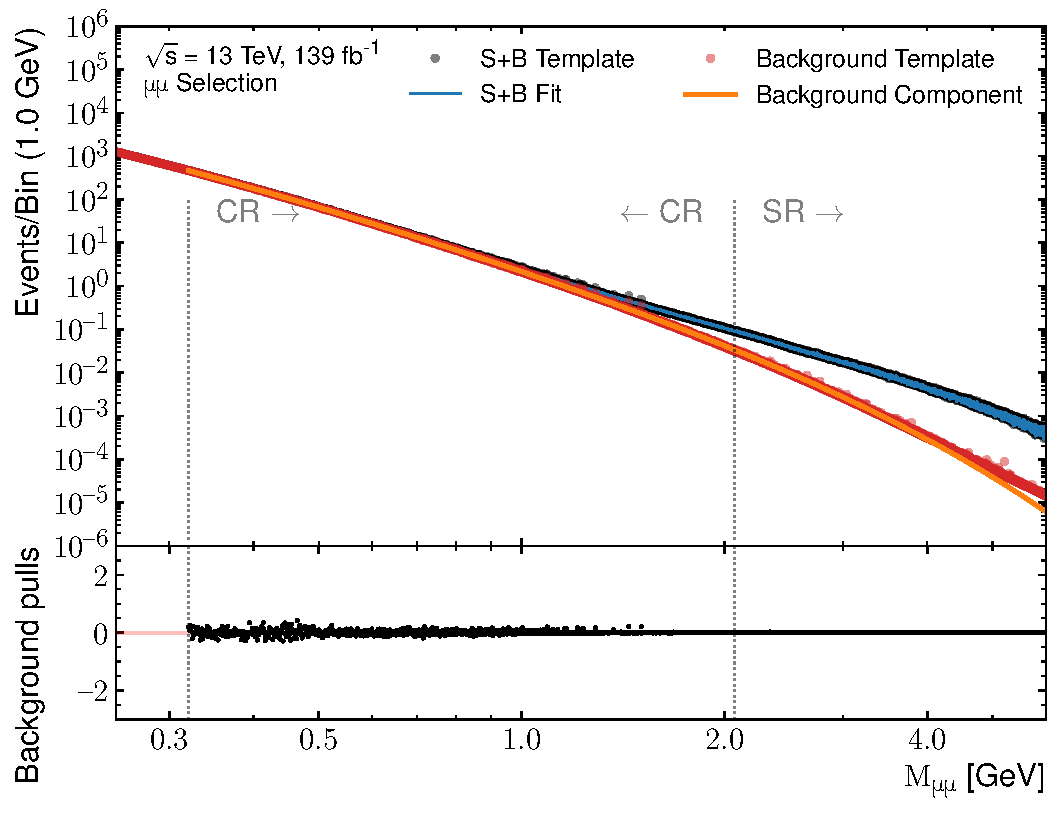
\includegraphics[width=\textwidth]{/Users/Deshan/Documents/PhD/thesis/Thesis/figures/analysis/bkgmodel/nominalFit-sb-const-LL-18-sbTrue-mm-.pdf}
        \label{fig:bkgmodel:sbfits2}
    \end{subfigure}
    \caption[Signal+Background fits to the signal+background template in the electron and muon channels]{Signal+background (S+B) fit to the simulated template injected with a CI signal at $\Lambda = \SI{26}{\tera\electronvolt}$ in the electron (left) and muon (right) channels shown in the top pad. The background template and the background component of the S+B fit is also shown. The bottom pad shows the pulls of the background component of the fit compared to the background template. The CR and SR boundaries are shown in the figure.}
    \label{fig:bkgmodel:sbfits}
\end{figure}

\subsection{Signal injection test}\label{sec:extrap:recovery}
Signal injection tests are used to validate the requirement that the signal+background fit model can provide an accurate background estimate, regardless of the presence of a signal in the CR. The robustness of the signal+background fit model is validated by quantifying the deflection of the fit model in the presence of an injected signal in the template. The background component of the signal+background fit model is fit to signal+background templates consisting of the MC background template injected with CI models in a range of $\Lambda$ value. The background expectation from the injected templates is compared to the background only template. 

\cref{fig:bkgmodel:injeeconst,fig:bkgmodel:injmmconst,fig:bkgmodel:injeedest,fig:bkgmodel:injmmdest} depict the injection tests for the electron and muon channel for the different chiral and interference models considered. The final CR and signal region choices are used to depict the performance of the signal+background model. The background estimation from the signal+background fit is compared at different injected signals. The Figures show that the background estimate does not change significantly in the presence of injected CI signals. Statistical fluctuations in the injected signals cause small discrepancies between background estimates, as seen in \cref{fig:bkgmodel:injeeconst}. The signals are injected from $\Lambda = \SI{18}{\tera\electronvolt}$ to \SI{40}{\tera\electronvolt}. 

\begin{figure}[h!]
    \centering
    \begin{subfigure}[b]{0.49\textwidth}
        \centering
        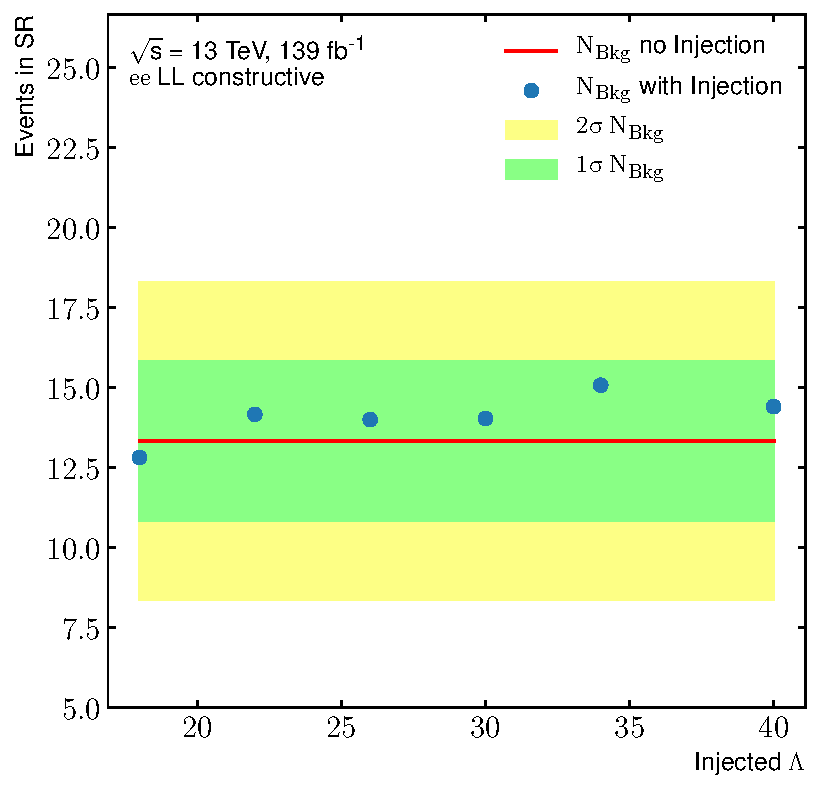
\includegraphics[width=\textwidth]{/Users/Deshan/Documents/PhD/thesis/Thesis/figures/analysis/bkgmodel/injections/injFlat-const-LL-ee.pdf}
        \label{fig:bkgmodel:injee1}
    \end{subfigure}
    \begin{subfigure}[b]{0.49\textwidth}
        \centering
        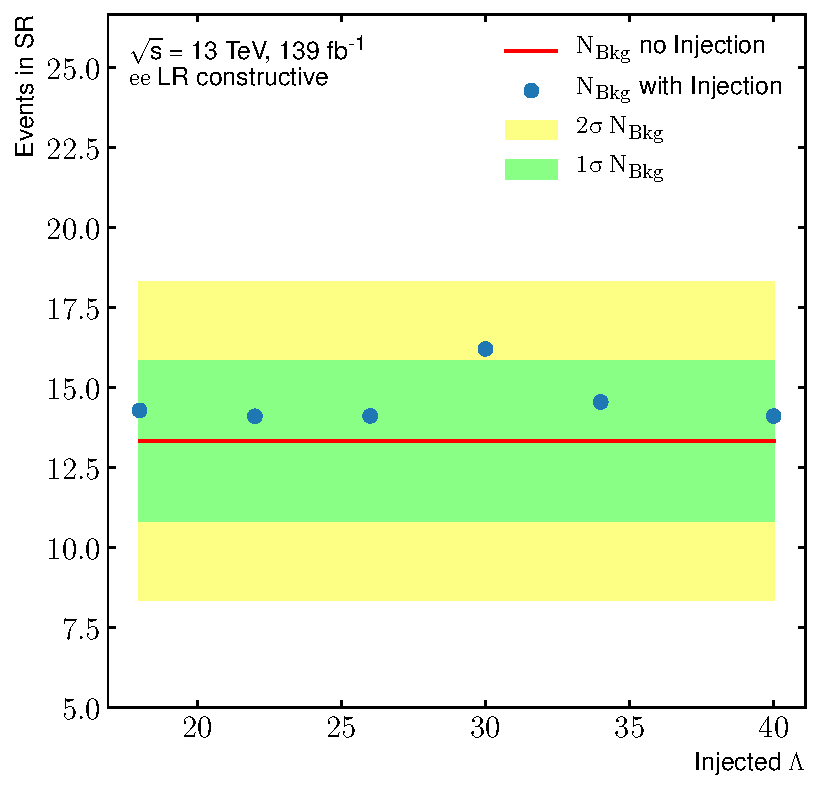
\includegraphics[width=\textwidth]{/Users/Deshan/Documents/PhD/thesis/Thesis/figures/analysis/bkgmodel/injections/injFlat-const-LR-ee.pdf}
        \label{fig:bkgmodel:injee3}
    \end{subfigure}
    \begin{subfigure}[b]{0.49\textwidth}
        \centering
        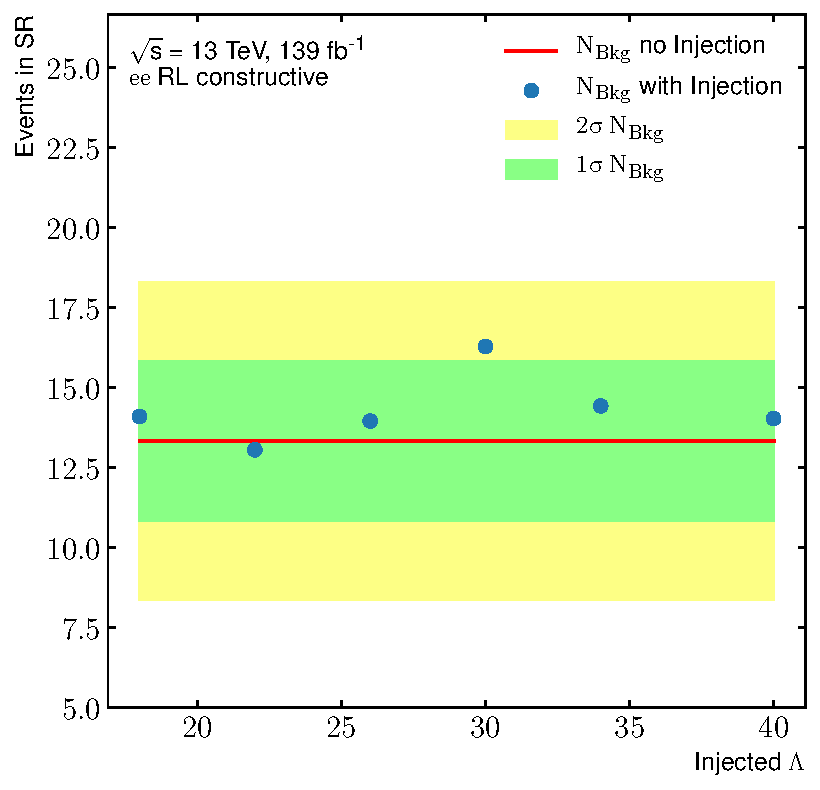
\includegraphics[width=\textwidth]{/Users/Deshan/Documents/PhD/thesis/Thesis/figures/analysis/bkgmodel/injections/injFlat-const-RL-ee.pdf}
        \label{fig:bkgmodel:injee5}
    \end{subfigure}
    \begin{subfigure}[b]{0.49\textwidth}
        \centering
        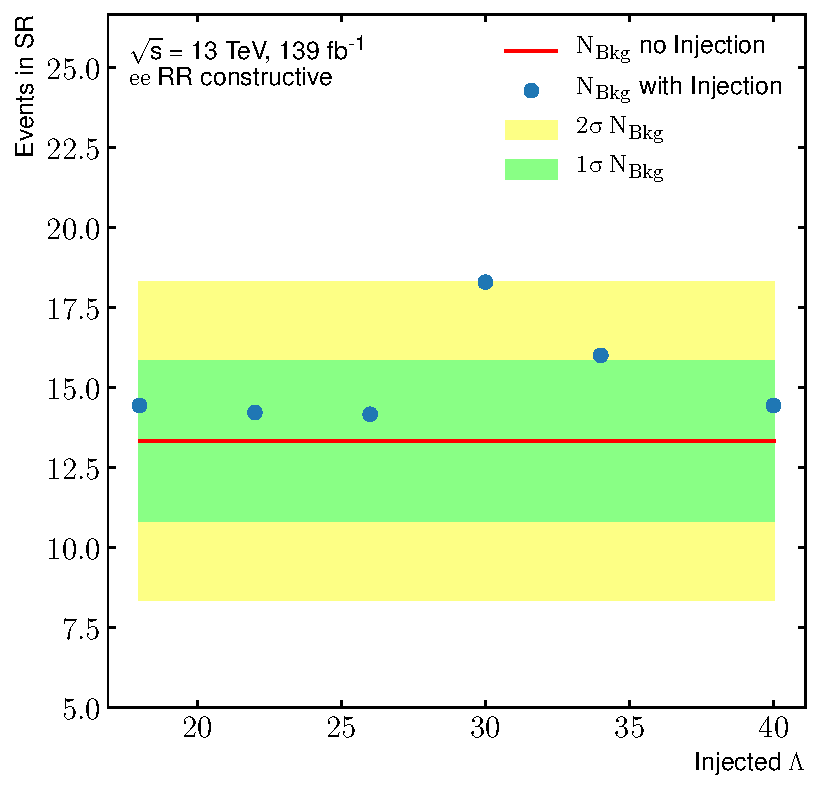
\includegraphics[width=\textwidth]{/Users/Deshan/Documents/PhD/thesis/Thesis/figures/analysis/bkgmodel/injections/injFlat-const-RR-ee.pdf}
        \label{fig:bkgmodel:injee7}
    \end{subfigure}
    \caption[Signal injection tests in the electron channel for constructive interference models]{Signal injection tests in the electron channel. The background expectation in the signal region for the signal+background fit model is compared for fits to the background template with injections of various chiral CI signals from $\Lambda = \SI{18}{\tera\electronvolt}$ to \SI{40}{\tera\electronvolt}. The LL, LR, RL, and RR chiral constructive interference models are injected. The background estimation from the fit to the background MC template with is associated uncertainty is also shown.}
    \label{fig:bkgmodel:injeeconst}
\end{figure}

\begin{figure}[h!]
    \centering
    \begin{subfigure}[b]{0.49\textwidth}
        \centering
        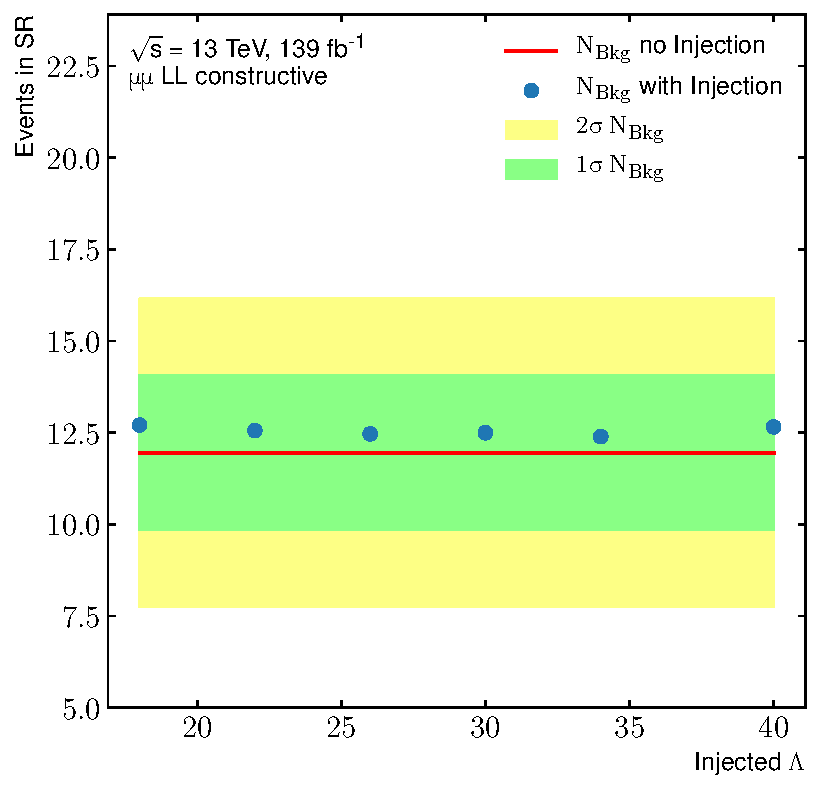
\includegraphics[width=\textwidth]{/Users/Deshan/Documents/PhD/thesis/Thesis/figures/analysis/bkgmodel/injections/injFlat-const-LL-mm.pdf}
        \label{fig:bkgmodel:injmm1}
    \end{subfigure}
    \begin{subfigure}[b]{0.49\textwidth}
        \centering
        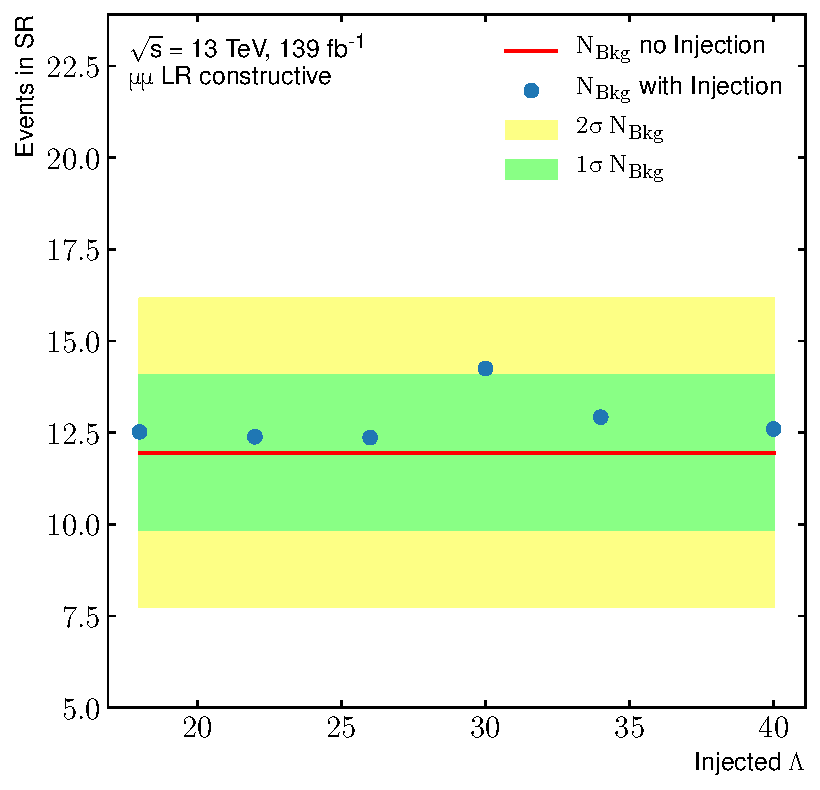
\includegraphics[width=\textwidth]{/Users/Deshan/Documents/PhD/thesis/Thesis/figures/analysis/bkgmodel/injections/injFlat-const-LR-mm.pdf}
        \label{fig:bkgmodel:injmm3}
    \end{subfigure}
    \begin{subfigure}[b]{0.49\textwidth}
        \centering
        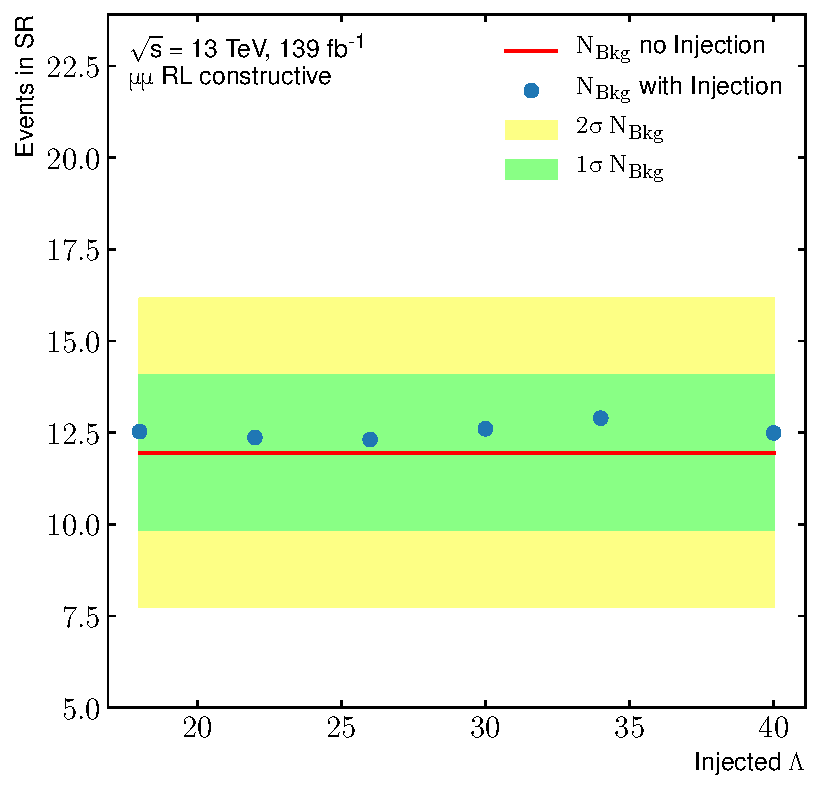
\includegraphics[width=\textwidth]{/Users/Deshan/Documents/PhD/thesis/Thesis/figures/analysis/bkgmodel/injections/injFlat-const-RL-mm.pdf}
        \label{fig:bkgmodel:injmm5}
    \end{subfigure}
    \begin{subfigure}[b]{0.49\textwidth}
        \centering
        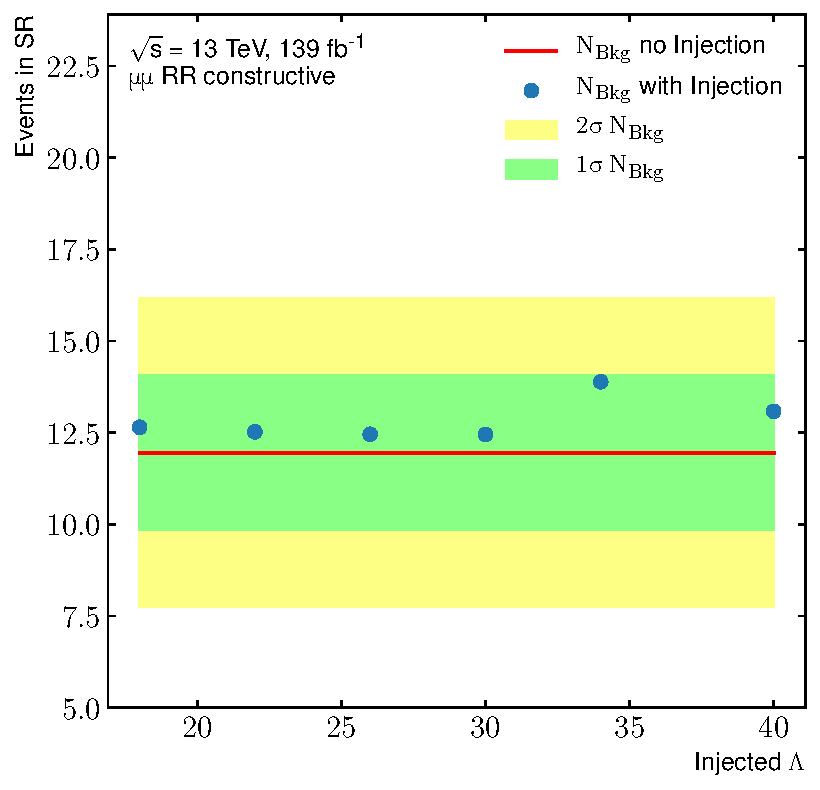
\includegraphics[width=\textwidth]{/Users/Deshan/Documents/PhD/thesis/Thesis/figures/analysis/bkgmodel/injections/injFlat-const-RR-mm.pdf}
        \label{fig:bkgmodel:injmm7}
    \end{subfigure}
    \caption[Signal injection tests in the muon channel for destructive interference models]{Signal injection tests in the muon channel. The background expectation in the signal region for the signal+background fit model is compared for fits to the background template with injections of various chiral CI signals from $\Lambda = \SI{18}{\tera\electronvolt}$ to \SI{40}{\tera\electronvolt}. The LL, LR, RL, and RR chiral destructive interference models are injected. The background estimation from the fit to the background MC template with is associated uncertainty is also shown.}
    \label{fig:bkgmodel:injmmconst}
\end{figure}

\begin{figure}[h!]
    \centering
    \begin{subfigure}[b]{0.49\textwidth}
        \centering
        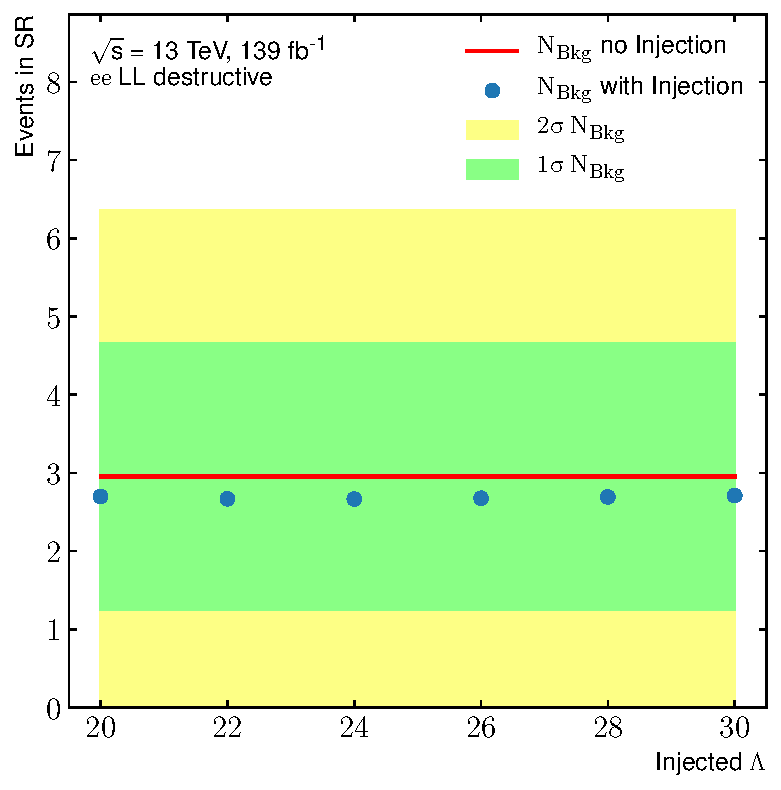
\includegraphics[width=\textwidth]{/Users/Deshan/Documents/PhD/thesis/Thesis/figures/analysis/bkgmodel/injections/injFlat-dest-LL-ee.pdf}
        \label{fig:bkgmodel:injee2}
    \end{subfigure}
    \begin{subfigure}[b]{0.49\textwidth}
        \centering
        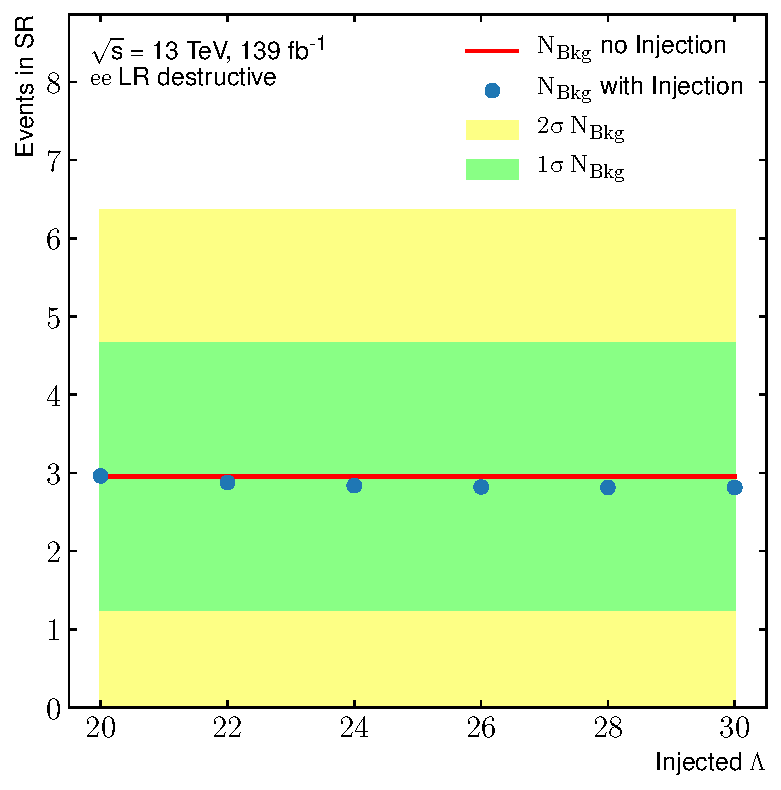
\includegraphics[width=\textwidth]{/Users/Deshan/Documents/PhD/thesis/Thesis/figures/analysis/bkgmodel/injections/injFlat-dest-LR-ee.pdf}
        \label{fig:bkgmodel:injee4}
    \end{subfigure}
    \begin{subfigure}[b]{0.49\textwidth}
        \centering
        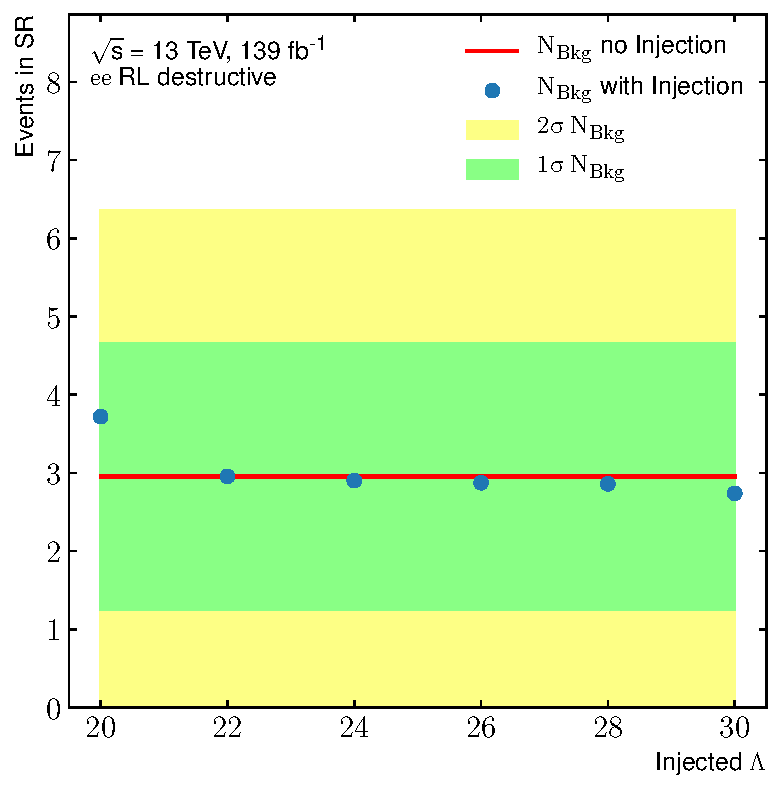
\includegraphics[width=\textwidth]{/Users/Deshan/Documents/PhD/thesis/Thesis/figures/analysis/bkgmodel/injections/injFlat-dest-RL-ee.pdf}
        \label{fig:bkgmodel:injee6}
    \end{subfigure}
    \begin{subfigure}[b]{0.49\textwidth}
        \centering
        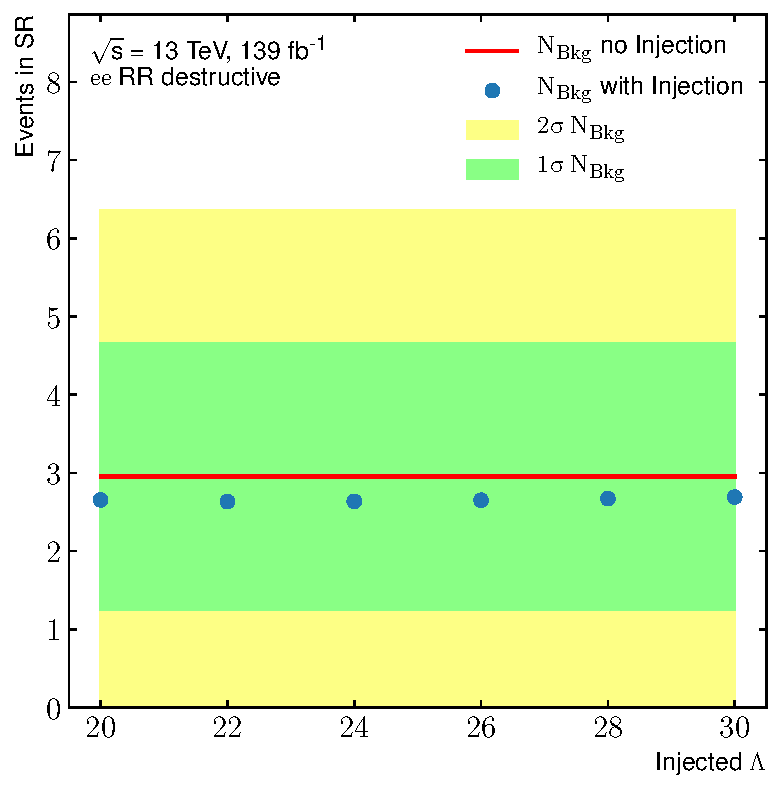
\includegraphics[width=\textwidth]{/Users/Deshan/Documents/PhD/thesis/Thesis/figures/analysis/bkgmodel/injections/injFlat-dest-RR-ee.pdf}
        \label{fig:bkgmodel:injee8}
    \end{subfigure}
    \caption[Signal injection tests in the electron channel for destructive interference models]{Signal injection tests in the electron channel. The background expectation in the signal region for the signal+background fit model is compared for fits to the background template with injections of various chiral CI signals from $\Lambda = \SI{18}{\tera\electronvolt}$ to \SI{40}{\tera\electronvolt}. The LL, LR, RL, and RR chiral constructive interference models are injected. The background estimation from the fit to the background MC template with is associated uncertainty is also shown.}
    \label{fig:bkgmodel:injeedest}
\end{figure}

\begin{figure}[h!]
    \centering
    \begin{subfigure}[b]{0.49\textwidth}
        \centering
        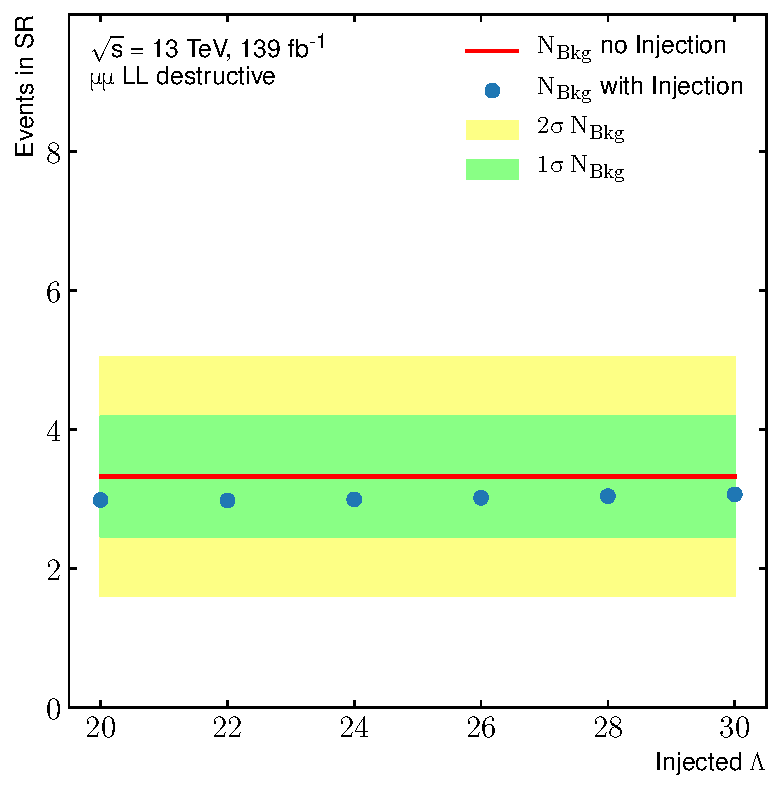
\includegraphics[width=\textwidth]{/Users/Deshan/Documents/PhD/thesis/Thesis/figures/analysis/bkgmodel/injections/injFlat-dest-LL-mm.pdf}
        \label{fig:bkgmodel:injmm2}
    \end{subfigure}
    \begin{subfigure}[b]{0.49\textwidth}
        \centering
        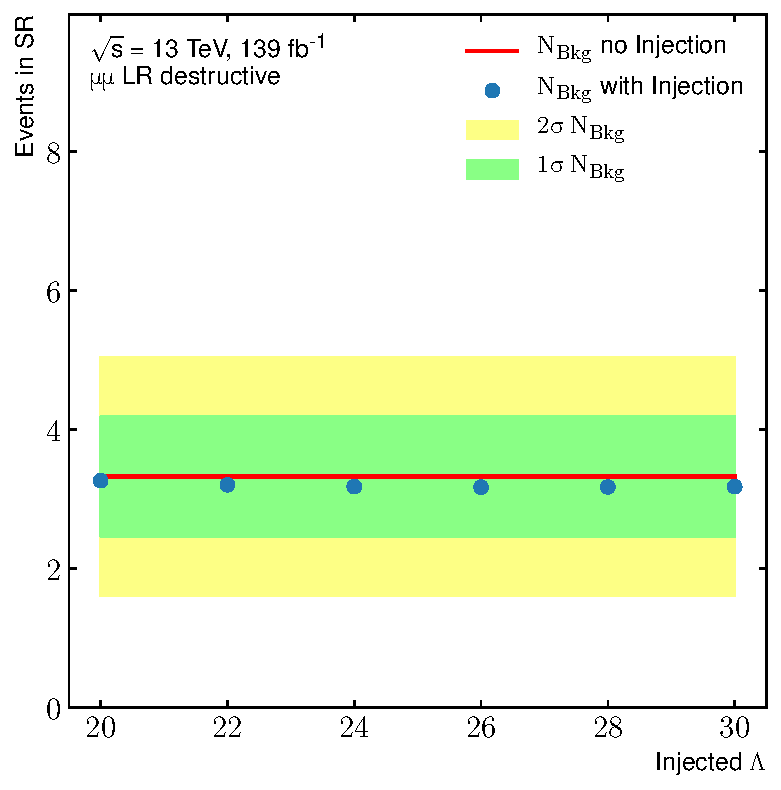
\includegraphics[width=\textwidth]{/Users/Deshan/Documents/PhD/thesis/Thesis/figures/analysis/bkgmodel/injections/injFlat-dest-LR-mm.pdf}
        \label{fig:bkgmodel:injmm4}
    \end{subfigure}
    \begin{subfigure}[b]{0.49\textwidth}
        \centering
        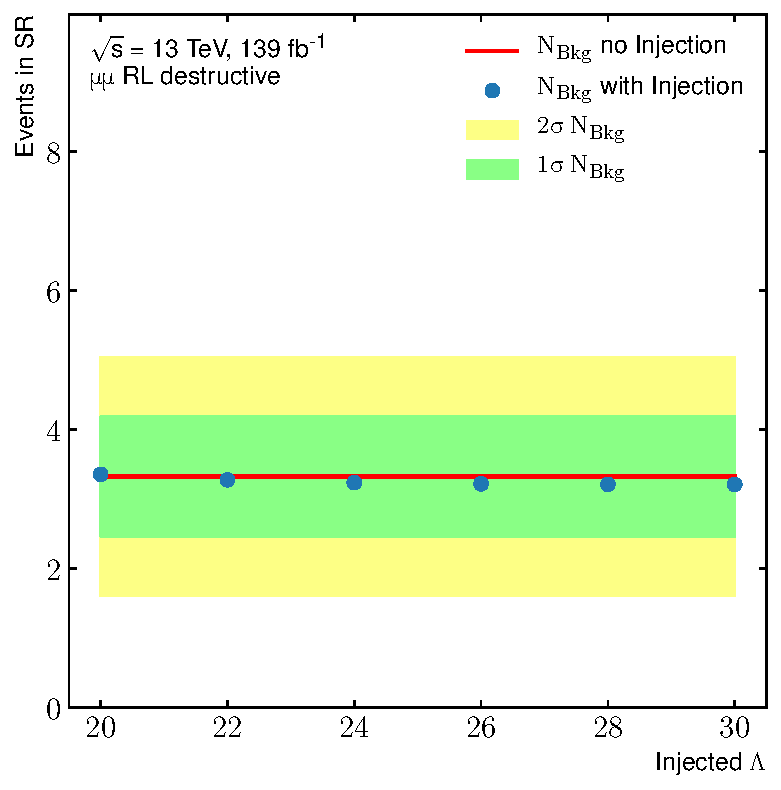
\includegraphics[width=\textwidth]{/Users/Deshan/Documents/PhD/thesis/Thesis/figures/analysis/bkgmodel/injections/injFlat-dest-RL-mm.pdf}
        \label{fig:bkgmodel:injmm6}
    \end{subfigure}
    \begin{subfigure}[b]{0.49\textwidth}
        \centering
        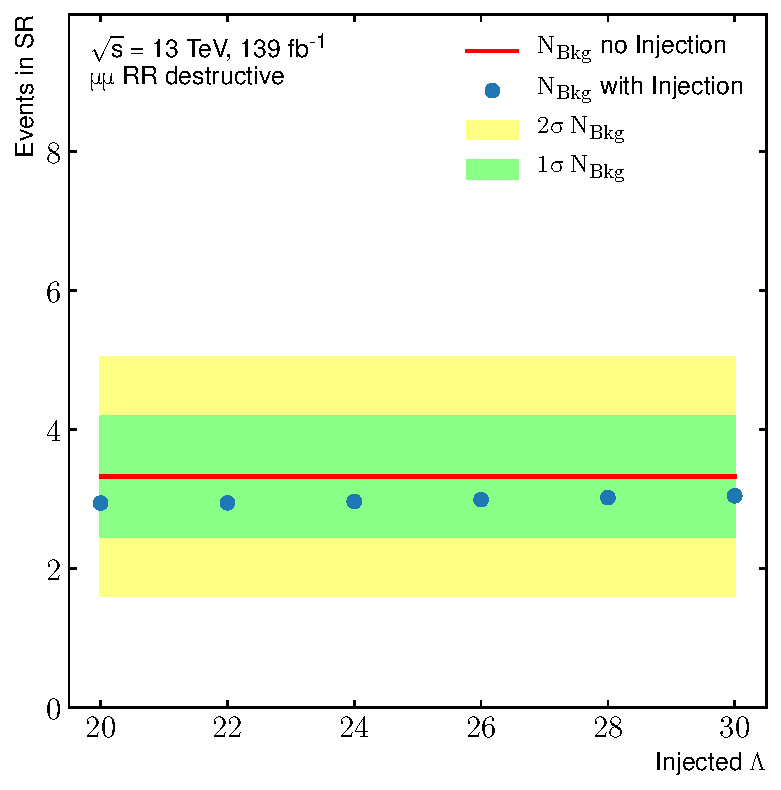
\includegraphics[width=\textwidth]{/Users/Deshan/Documents/PhD/thesis/Thesis/figures/analysis/bkgmodel/injections/injFlat-dest-RR-mm.pdf}
        \label{fig:bkgmodel:injmm8}
    \end{subfigure}
    \caption[Signal injection tests in the muon channel for destructive interference models]{Signal injection tests in the muon channel. The background expectation in the signal region for the signal+background fit model is compared for fits to the background template with injections of various chiral CI signals from $\Lambda = \SI{18}{\tera\electronvolt}$ to \SI{40}{\tera\electronvolt}. The LL, LR, RL, and RR chiral constructive interference models are injected. The background estimation from the fit to the background MC template with is associated uncertainty is also shown.}
    \label{fig:bkgmodel:injmmdest}
\end{figure}

\clearpage

\section{Optimisation of control and signal regions}\label{sec:extrap:optimisation}
The optimisation procedure attempts to maximise the expected sensitivity to CI signals by varying the CR and SR boundaries. For each CI signal model and channel in consideration the lower and upper boundary of the CR ($\mathrm{CR}_{\mathrm{min}}$ and $\mathrm{CR}_{\mathrm{max}}$), and the lower boundary of the SR ($\mathrm{SR}_{\mathrm{min}}$) are varied to maximise sensitivity to CI signals. 

The expected limit is used to test the sensitivity to the CI models. The expected limit includes the \ISSU and \STATU uncertainties, described in \cref{sec:extrap:uncertainties}, and is calculated following the procedure described in \cref{chap:stats}. Optimisation based solely on the expected limit would prefer CRs that extend to higher masses, as shown in \cref{sec:extrap:ststu}. However, extending the CR to high-mass may result in a possible bias to the background expectation from signals present in data. This is addressed by introducing a second criteria based on minimising the linearity of the signal injection tests. The linearity criteria considers the performance of the recovery of signal events across a range of plausible CI signals injected to the MC background template, and is defined as: 
\begin{equation}
    \label{eq:linearity}
    \begin{aligned}
        \mathrm{Linearity} = \sum^{\Lambda = 18}_{\Lambda = \infty} \frac{N_{S,\mathrm{rec},\Lambda}}{N_{S,\mathrm{inj},\Lambda}}  \frac{1}{\mathrm{N}},
    \end{aligned}
\end{equation}

where $\Lambda$ is the CI energy scale in the injected MC template that is fit. $\Lambda = \infty$ corresponds to the background-only MC template, while $\Lambda = 18$ corresponds to a \SI{18}{\tera\electronvolt} CI signal injected. $N_{S,\mathrm{inj},\Lambda}$ is the number of injected signal events in the SR. $N_{S,\mathrm{rec},\Lambda}$ corresponds to the recovered number of signals events, defined as the difference between integrals of the signal+background template that is fit and the background expectation of the fit and extrapolation in the SR. N is the number of different signals that are injected, used to normalise the linearity to unity. The signal+background fit model is used for the linearity tests. 

A combination of both the expected limit and the linearity is used to pick a final CR and SR configuration. The expected limit naturally prefers CR configurations that extend to higher invariant mass, whereas, the linearity is minimum for CR configurations at lower invariant mass. Therefore, a balance between the expected limit and linearity is required for an optimal CR and SR configuration. The different chiral and interference CI signal models are considered in the optimisation. The chiral models correspond to LL, LR, RL, and RR, and the interference models considered are either constructive and destructive. In the destructive interference cases, if the SR includes a significant contribution from the destructive interference component of the CI signal shape, the integral number of expected events in the SR is reduced. Therefore, the optimisation procedure allows for a gap between the CR and SRs to avoid this effect. Additionally, the inclusion of the destructive component of the signal shape in the CR results in a poor linearity when performing the signal injection tests. 

Each chirality and interference choice of the CI model is tested with an independent CR and SR configuration. It is found that for models with destructive interference a mass gap of \SI{1320}{\giga\electronvolt} is preferred by the optimisation procedure, while for the constructive interference models, the optimal $\mathrm{CR}_{\mathrm{max}}$ coincides with $\mathrm{SR}_{\mathrm{min}}$. Similar performance is shown for the resulting ranges for the chirality options at the level of few tens of \SI{}{\giga\electronvolt}. Therefore, the ranges for the different chiral models are merged, as shown in \cref{tab:bkgModel:massRanges} to simply the subsequent procedures. The function given is \cref{eq:fitfunc} is used to measure the background estimate in the SR for these configurations. 

\begin{table}[htp]
    \centering
    \begin{tabular}{l | c c c | c c c}
    \toprule
    Channel & \multicolumn{3}{c|}{Constructive interference} & \multicolumn{3}{c}{Destructive interference} \\
     & $\mathrm{CR}_{\mathrm{min}}$ & $\mathrm{CR}_{\mathrm{max}}$ & $\mathrm{SR}_{\mathrm{min}}$ & $\mathrm{CR}_{\mathrm{min}}$ & $\mathrm{CR}_{\mathrm{max}}$ & $\mathrm{SR}_{\mathrm{min}}$ \\
    \hline
    \ee & 280 & 2200 & 2200 & 310 & 1450 & 2770 \\
    \hline
    \mumu & 310 & 2070 & 2070 & 320 & 1250 & 2570 \\
    \bottomrule
    \end{tabular}
    \label{tab:bkgModel:massRanges}
    \caption{CR and SR ranges (in units of \SI{}{\giga\electronvolt}). For all configurations $\mathrm{SR}_{\mathrm{min}} = \SI{6000}{\giga\electronvolt}$.}
\end{table}

\subsection{Validation of the control region}
The robustness of the background estimate resulting from the fit to the final CR configurations chosen is also tested. The background estimate from the background only fit, and extrapolation in data for a given CR and SR region configuration is required to be unaffected by the possible contamination of a signal in the CR. Therefore, the signal+background model is used to validate the background-only fit and CR choice. The tests are performed on data once a CR and SR region choice has been chosen following the procedure described in \cref{sec:extrap:optimisation}. 

For a given CR, both the background only and signal+background functions are fit and the background only components of the signal+background fit is compared to the background only model. If the two background estimates do not differ significantly, then it can be concluded that there is no significant signal contribution present in the CR to bias the background-only fit. A difference  more significant than the uncertainty on the background estimate from the signal+background fit is considered to be large enough to invalidate a CR choice. Both in the presence and absence of signal, the background component of the signal+background fits are not deflected significantly. 

If a significant difference is observed between the two background estimates, then it is concluded that the control region includes an invariant mass range where a signal can impact the background-only fit. It can be concluded that due to expected the shape of the CI signals, the bias from the signals is a consequence the CR extending into high-mass regions where the CI signals start to dominate. Therefore, the CR upper edge can be lowered iteratively, each time checking the background estimates from the two fit functions until they agree. A significant difference between the background estimates from the two fit functions is only expected in data only if there is CI or other non-resonant signals present. 

The test of the compatibility of the signal+background and background only fits is shown in \cref{fig:bkgmodel:fitsbplusb} for the final CR and SR choices. The integrated number of background events in the SR from each fit is shown for the CR and SR configurations. The fits are performed on data once the CR and SR choices have been finalised. This example depicts a good agreement between the two fit models. The uncertainty shown corresponds to the uncertainty on the background estimate from the signal+background fit. Any difference observed between the two background estimates will be used as an additional uncertainty on the background estimate. Further detail on the estimation of background model uncertainties are given in \cref{sec:extrap:uncertainties}. 

The background estimate resulting from the two fit models fitting a data with an injected signal in an invalid CR choice is shown in \cref{fig:bkgmodel:fitsbplusbbad}. A CI signal corresponding to $\Lambda = \SI{18}{\tera\electronvolt}$ is injected into the data, and the CR region moved into high invariant-mass to exaggerate the effects on the background estimate. The background estimate from the background only fit is significantly deflected due to an excess of signal events in the CR.

\begin{figure}[h!]
    \centering
    \begin{subfigure}[b]{0.49\textwidth}
        \centering
        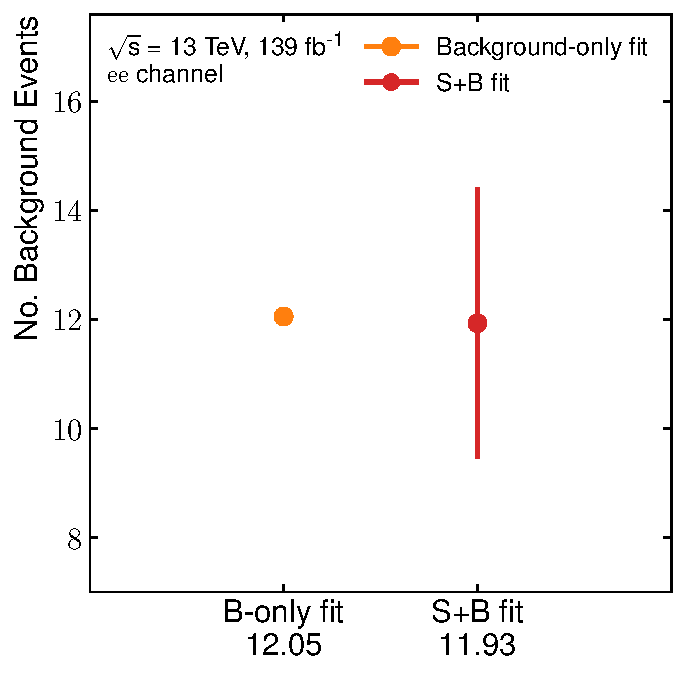
\includegraphics[width=\textwidth]{/Users/Deshan/Documents/PhD/thesis/Thesis/figures/analysis/bkgmodel/nbkg-LL-const-ee.pdf}
        \label{fig:bkgmodel:fitsbplusb1}
    \end{subfigure}
    \begin{subfigure}[b]{0.49\textwidth}
        \centering
        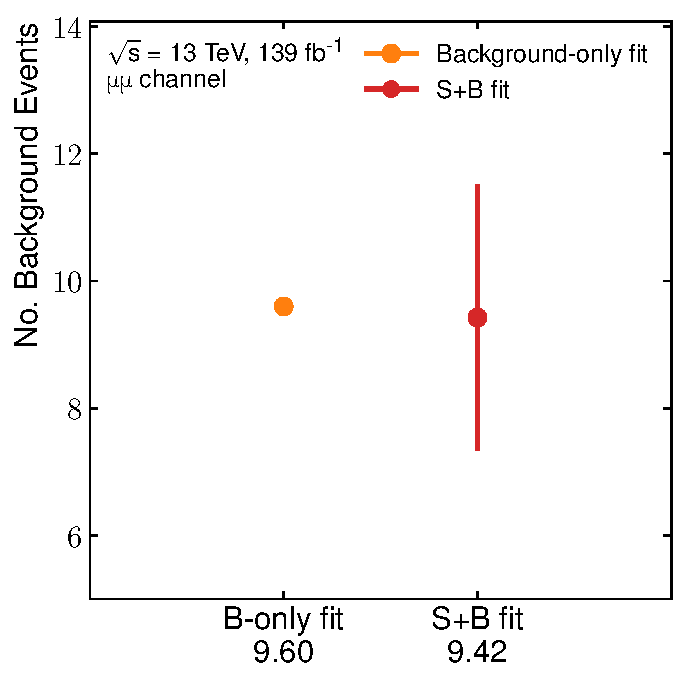
\includegraphics[width=\textwidth]{/Users/Deshan/Documents/PhD/thesis/Thesis/figures/analysis/bkgmodel/nbkg-LL-const-mm.pdf}
        \label{fig:bkgmodel:fitsbplusb2}
    \end{subfigure}
    \begin{subfigure}[b]{0.49\textwidth}
        \centering
        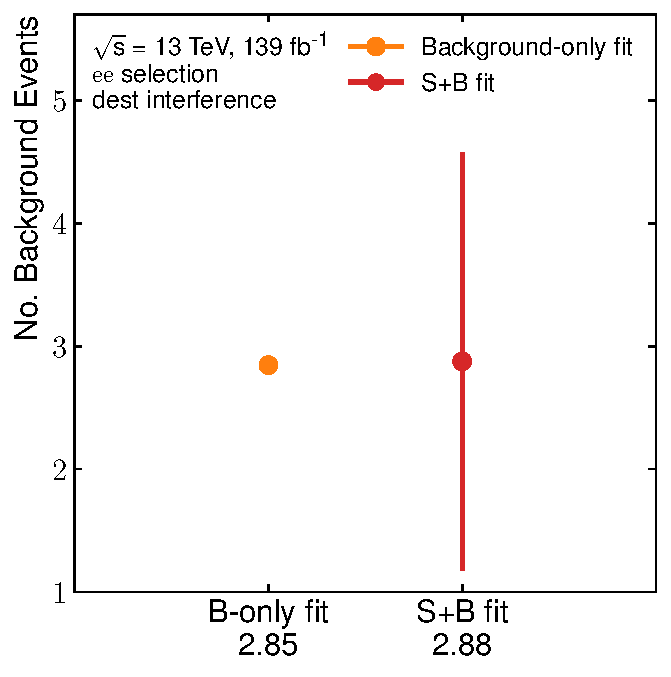
\includegraphics[width=\textwidth]{/Users/Deshan/Documents/PhD/thesis/Thesis/figures/analysis/bkgmodel/nbkg-LL-dest-ee.pdf}
        \label{fig:bkgmodel:fitsbplusb3}
    \end{subfigure}
    \begin{subfigure}[b]{0.49\textwidth}
        \centering
        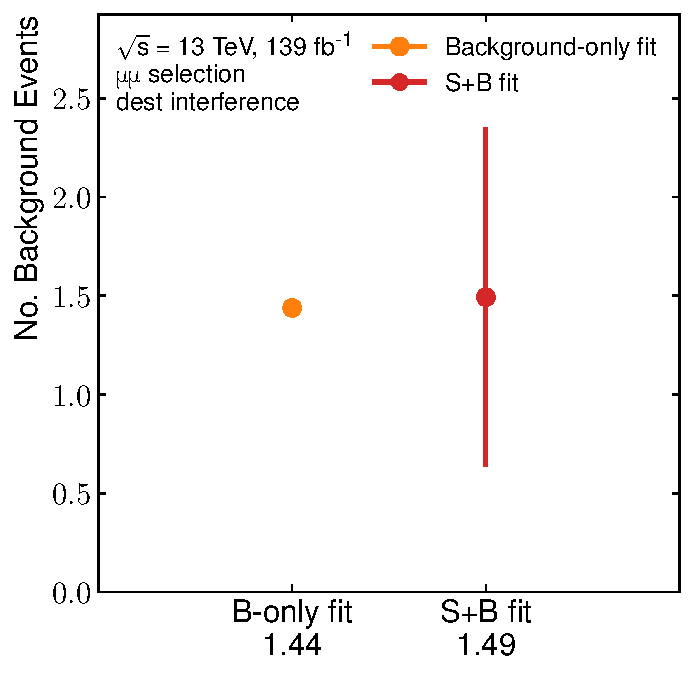
\includegraphics[width=\textwidth]{/Users/Deshan/Documents/PhD/thesis/Thesis/figures/analysis/bkgmodel/nbkg-LL-dest-mm.pdf}
        \label{fig:bkgmodel:fitsbplusb4}
    \end{subfigure}
    \caption[Background estimation comparisons of the signal+background fit and background only fit]{Number of background events in the signal region from the background only fit and the signal+background (S+B) fit on data in the constructive (top) and destructive (bottom) interference signal regions for the electron channel (left) and muon channel (right). The uncertainty on the background estimate is shown for background only fit. The number of background events from each fit is shown on the x-axis.}
    \label{fig:bkgmodel:fitsbplusb}
\end{figure}

\begin{figure}[h!]
    \centering
    \begin{subfigure}[b]{0.49\textwidth}
        \centering
        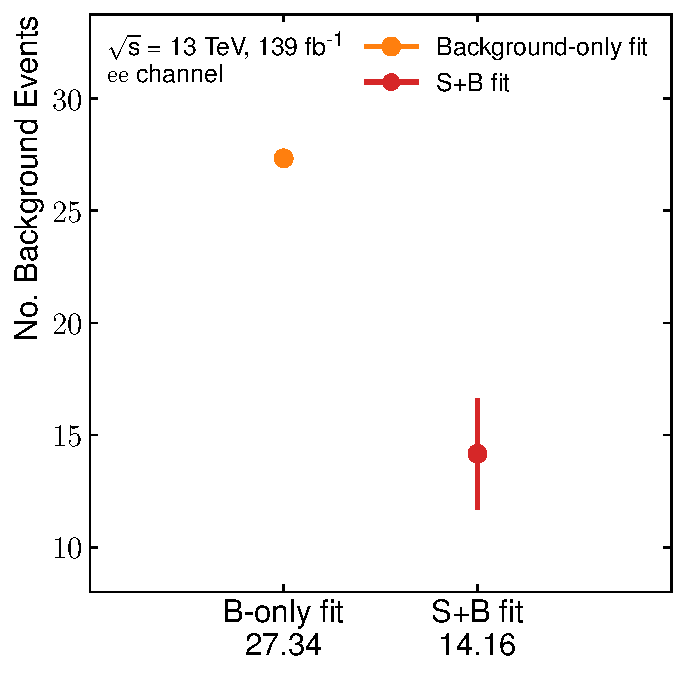
\includegraphics[width=\textwidth]{/Users/Deshan/Documents/PhD/thesis/Thesis/figures/analysis/bkgmodel/nbkg-LL-const-ee-bad.pdf}
        \label{fig:bkgmodel:fitsbplusb1bad}
    \end{subfigure}
    \begin{subfigure}[b]{0.49\textwidth}
        \centering
        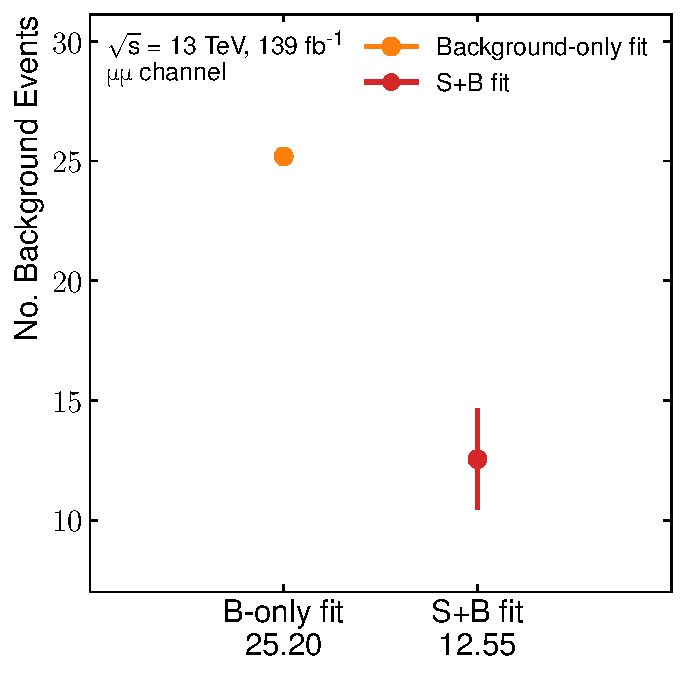
\includegraphics[width=\textwidth]{/Users/Deshan/Documents/PhD/thesis/Thesis/figures/analysis/bkgmodel/nbkg-LL-const-mm-bad.pdf}
        \label{fig:bkgmodel:fitsbplusb2bad}
    \end{subfigure}
    \caption[Background estimation comparisons of the signal+background fit and background only fit in an invalid CR choice.]{Number of background events in the signal region from the background only fit and the signal+background (S+B) fit on data with an injected CI signal with $\Lambda = \SI{18}{\tera\electronvolt}$, for the electron channel (left) and muon channel (right). The uncertainty on the background estimate is shown for background only fit. The number of background events from each fit is shown on the x-axis.}
    \label{fig:bkgmodel:fitsbplusbbad}
\end{figure}

\section{Uncertainties}\label{sec:extrap:uncertainties}
Quantifying the uncertainties associated with the background modelling has been a vital part of the analysis. The uncertainties related to the background modelling in the SR results from three sources described below. Experimental uncertainties on the signal model are also discussed in this section. The uncertainties are calculated for each CR and SR configuration used in the analysis. The background only fit model is used to determine the uncertainties on the background estimate. 

\subsection{Background estimate uncertainties}

\subsubsection{Induced spurious-signal uncertainty}
For a given underlying PDF that generates an invariant mass spectrum, the extrapolation from the low-mass CR to the high-mass signal region will naturally deviate from the underlying distribution, resulting in an excess or deficit compared to the background template. The \emph{induced spurious-signal} uncertainty (\ISSU) quantifies the agreement to which the background fit model, when extrapolated to the SR can induce a signal-like excess or deficit. 

The underlying background distribution in data is not known accurately. A \ISSU measurement made on the template from only the nominal PDF would assume the underlying distribution to be known precisely. Therefore, the theoretical uncertainties associated with the nominal PDF choice described in \cref{sec:sysmc:theory} are also considered in the \ISSU measurement. Additionally, due to detector and reconstruction effects on the simulated MC template, the experimental uncertainties, described in \cref{sec:sysmc:exp}, are also considered. 

The \ISSU is measured on the nominal MC background, and its systematic variations. An ensemble of possible simulated shapes are created scaling the nominal simulated background template by a linear combination of all of its systematic uncertainties. Each uncertainty is scaled by a Gaussian factor in the range [-1,1], summed together, and used to scale the simulated background shape to produce a toy distribution. \cref{eq:issutoy} outlines the procedure used to construct each toy background shape. 
\begin{equation}
    \label{eq:issutoy}
    \begin{aligned}
        & Toy = \sum_{i} N_{bkg,i} + \sum_{j} \left(\delta_{i,j} * \alpha_{j}\right), \\
        & \alpha_j = \mathrm{Gaus}(\sigma=1,\overline{x}=0),
    \end{aligned}
\end{equation}
where $N_{bkg,i}$ is the number of background events in invariant mass bin \emph{i} for the nominal simulated background distribution. $\delta_{i,j}$ is the uncertainty for background uncertainty \emph{j}, and $\alpha_j$ a factor sampled from a gaussian distribution used to scale each uncertainty.

The resulting toy shape is fitted and extrapolated to the SR. The difference between the integral of the extrapolation and the toy background in the SR is taken as the induced spurious signal per toy. The induced spurious-signal is calculated for each toy in the ensemble of toys, producing a distribution for induced spurious-signal values. The sum in quadrature of the mean and standard deviation of the induced spurious-signal distribution is taken as the \ISSU. 

The induced spurious signal distributions, as event yields in the SR, for the CR and SRs considered in the analysis is shown in \cref{fig:bkgmodel:issu}. 10000 toy uncertainty templates are made and fit using the background-only fit model. The induced spurious signal for each toy is calculated to form the distribution. The standard deviation and the mean are calculated from the spurious signal distribution to determine the \ISSU. 10000 toys is deemed appropriate as the mean, and standard deviation of the distributions are found to be consistent stable up to 0.001 when comparing with distributions with 9000 toys.

\begin{figure}[h!]
    \centering
    \begin{subfigure}[b]{0.49\textwidth}
        \centering
        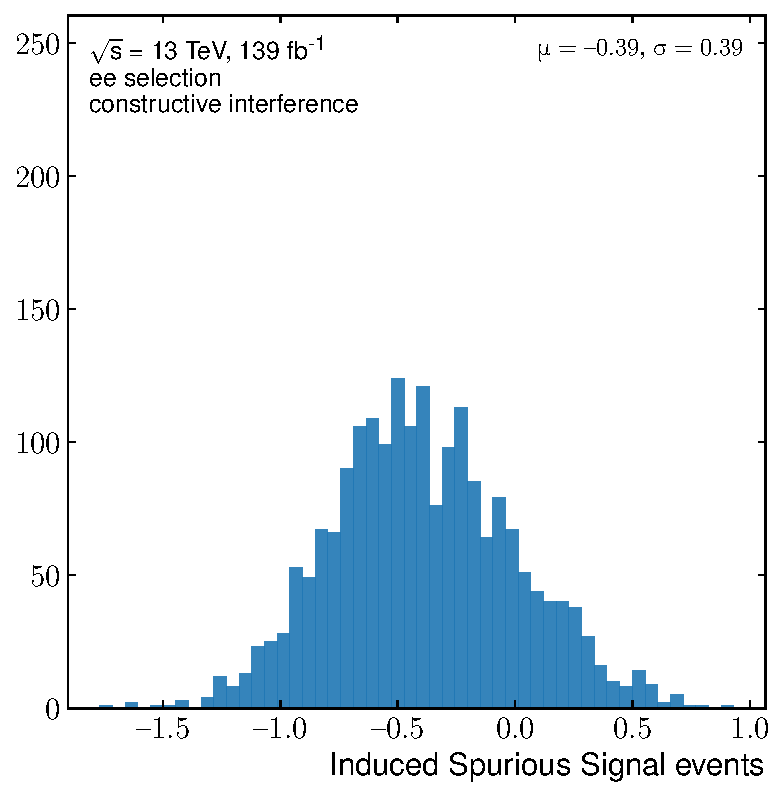
\includegraphics[width=\textwidth]{/Users/Deshan/Documents/PhD/thesis/Thesis/figures/analysis/bkgmodel/uncertainties/toyNSSDist-ee-const-all-noGaus.pdf}
        \label{fig:bkgmodel:issu1}
    \end{subfigure}
    \begin{subfigure}[b]{0.49\textwidth}
        \centering
        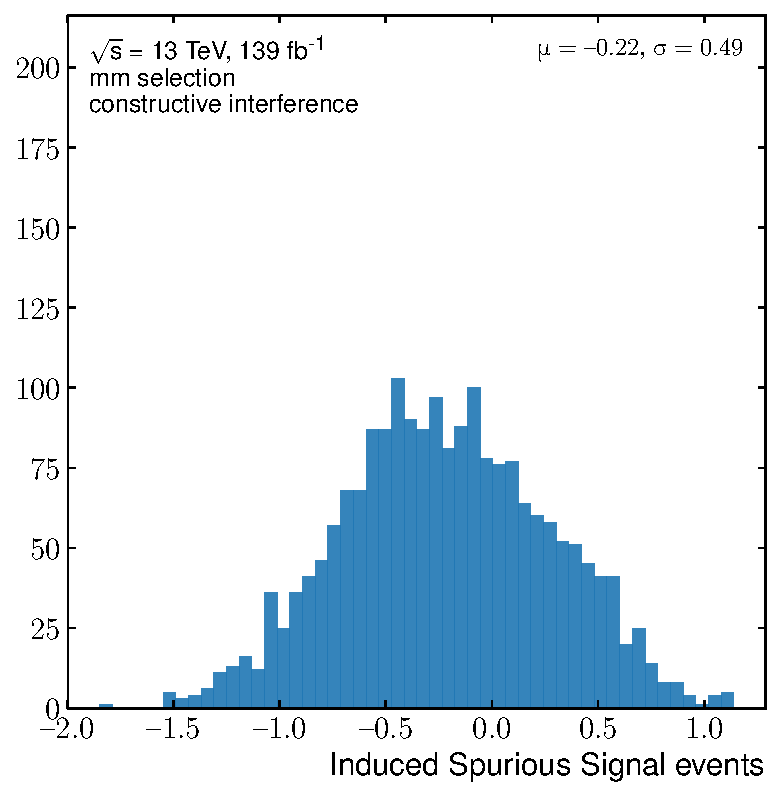
\includegraphics[width=\textwidth]{/Users/Deshan/Documents/PhD/thesis/Thesis/figures/analysis/bkgmodel/uncertainties/toyNSSDist-mm-const-all-noGaus.pdf}
        \label{fig:bkgmodel:issu2}
    \end{subfigure}
    \begin{subfigure}[b]{0.49\textwidth}
        \centering
        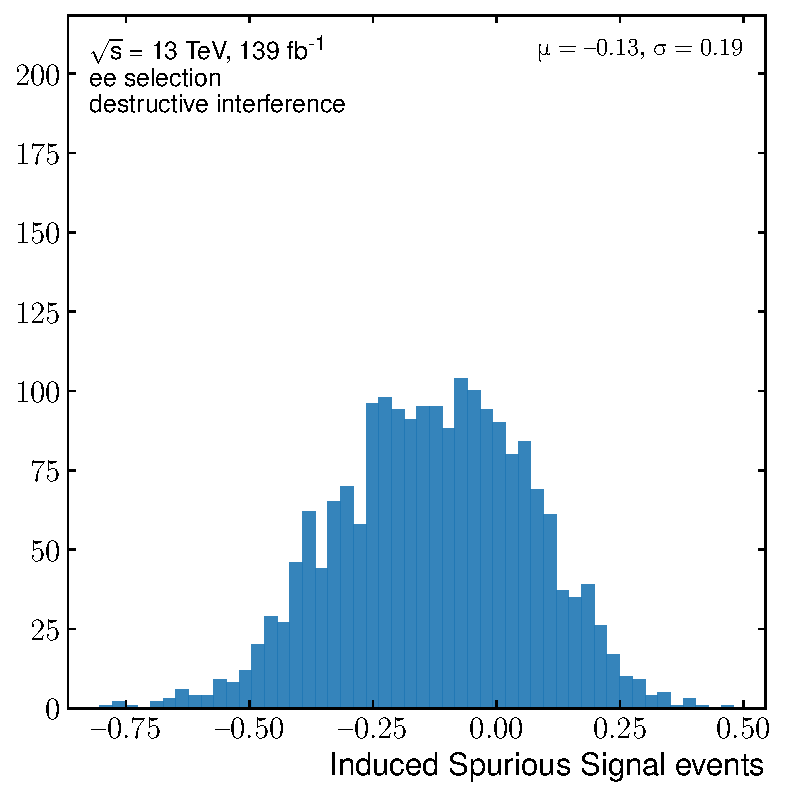
\includegraphics[width=\textwidth]{/Users/Deshan/Documents/PhD/thesis/Thesis/figures/analysis/bkgmodel/uncertainties/toyNSSDist-ee-dest-all-noGaus.pdf}
        \label{fig:bkgmodel:issu3}
    \end{subfigure}
    \begin{subfigure}[b]{0.49\textwidth}
        \centering
        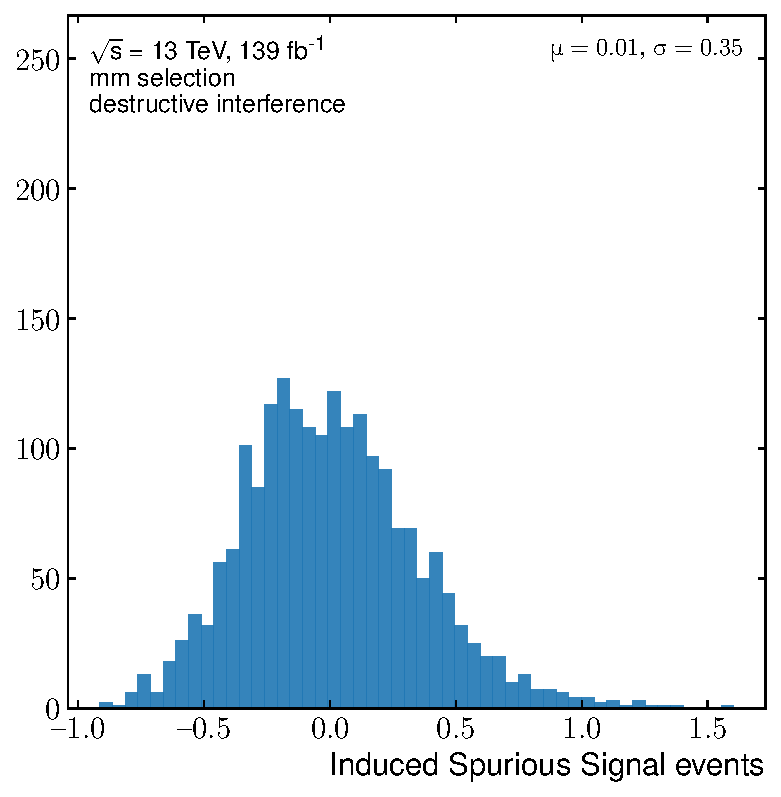
\includegraphics[width=\textwidth]{/Users/Deshan/Documents/PhD/thesis/Thesis/figures/analysis/bkgmodel/uncertainties/toyNSSDist-mm-dest-all-noGaus.pdf}
        \label{fig:bkgmodel:issu4}
    \end{subfigure}
    \caption[Induced spurious signal distributions from fits to toy uncertainties.]{Distribution of induced spurious signal values, as number of events, from fits to toy uncertainty shapes. The distributions for the constructive (top) and destructive (bottom) signal regions in the electron (left) and muon (right) channels are included. The mean and standard deviation for the induced spurious signal distribution is also shown.}
    \label{fig:bkgmodel:issu}
\end{figure}

\subsubsection{Statistical uncertainty of fit}\label{sec:extrap:ststu}
Statistical fluctuations in data can lead to variations of the fitted background model in the CR. The resulting variations of the fitted background impact the extrapolated background in the SR. The impact of the statical fluctuations, \STATU, is estimated from fitting an ensemble of toy datasets. The invariant mass distribution resulting from the background fit to the data in the CR is used as a probability density function, from which an ensemble of toy datasets are generated by varying each bin using a Poisson distribution. The background model is fit to each of the toy datasets in the ensemble individually, extrapolated and integrated in the SR. The difference between integral of the toy template in the SR and the fit is calculated. The standard deviation of the distribution of differences is taken as the \STATU. 

The distribution of the toy background estimates is confirmed to be centred at the nominal induced spurious signal, indicating no bias in the estimation of the uncertainty. The sufficient number of toy background distributions are produced to achieve a precise measurement of the uncertainty. The \STATU is the dominant uncertainty in the fit and extrapolation. Extending the CR boundary to higher mass constrains the fit with more information and results in smaller variations due to statistical fluctuations. A detailed study of the optimisation of the CR choice is discussed in \cref{sec:extrap:optimisation}.

\cref{fig:bkgmodel:toyss} depicts the distribution of differences between the background estimate in the SR from the fit to 10000 background toys and the integral of the background toy in the SR. These distributions are centred around the induced spurious signal from the nominal template as expected. The standard deviation of the distribution is taken as the \STATU. The \ISSU is calculated for each SR configuration considered in the analysis. The standard deviation of the distribution is confirmed to be consistent at 10000 toys. 

\begin{figure}[h!]
    \centering
    \begin{subfigure}[b]{0.49\textwidth}
        \centering
        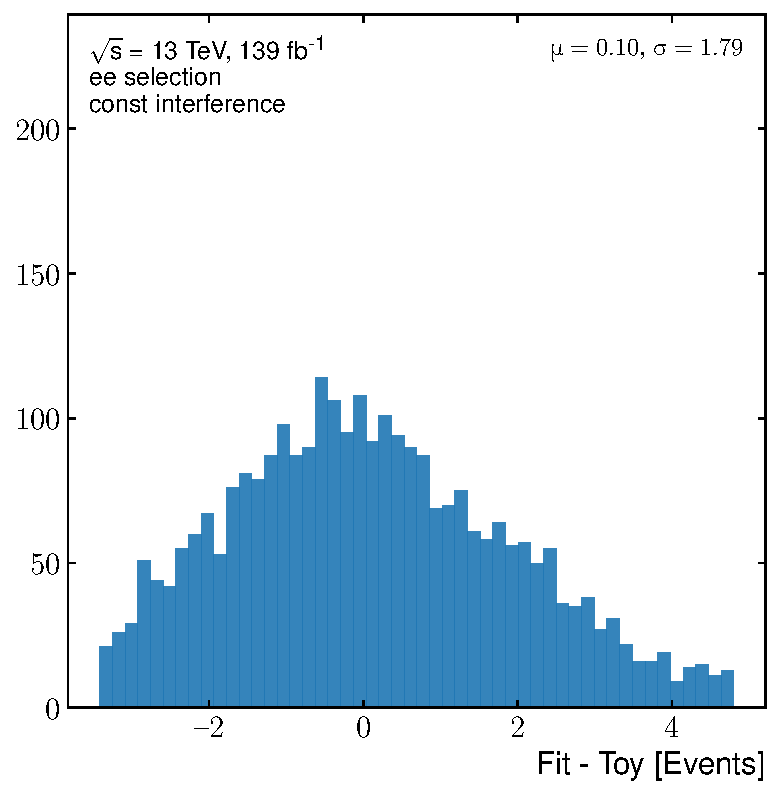
\includegraphics[width=\textwidth]{/Users/Deshan/Documents/PhD/thesis/Thesis/figures/analysis/bkgmodel/uncertainties/fitSs-ee-const.pdf}
        \label{fig:bkgmodel:toyss1}
    \end{subfigure}
    \begin{subfigure}[b]{0.49\textwidth}
        \centering
        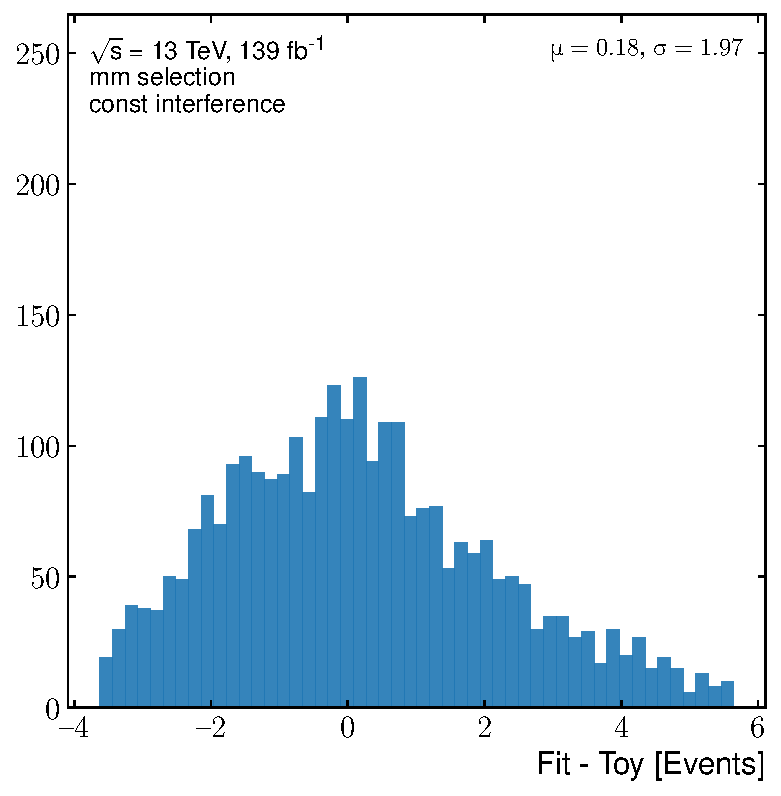
\includegraphics[width=\textwidth]{/Users/Deshan/Documents/PhD/thesis/Thesis/figures/analysis/bkgmodel/uncertainties/fitSs-mm-const.pdf}
        \label{fig:bkgmodel:toyss2}
    \end{subfigure}
    \begin{subfigure}[b]{0.49\textwidth}
        \centering
        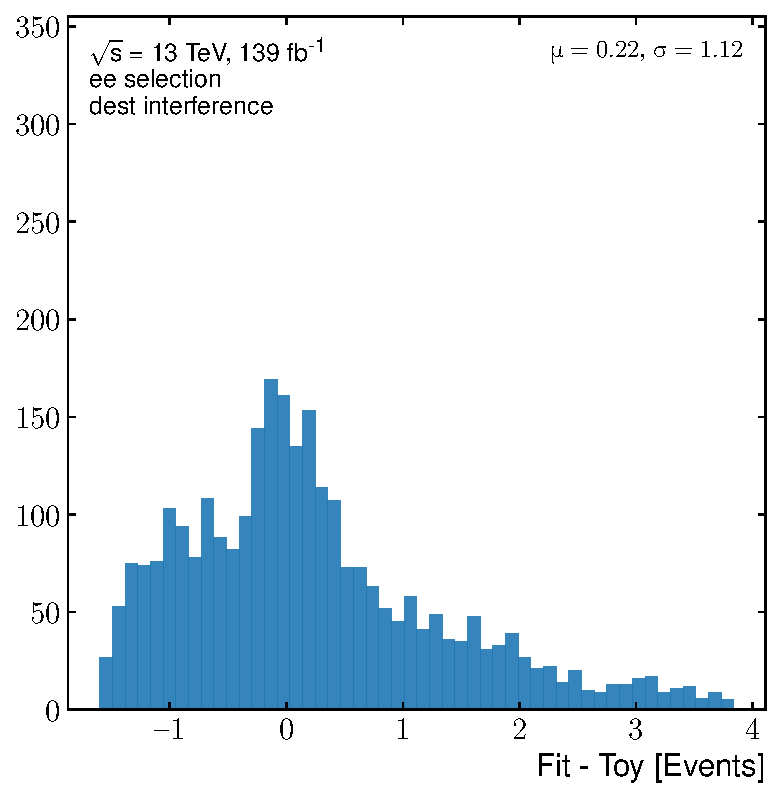
\includegraphics[width=\textwidth]{/Users/Deshan/Documents/PhD/thesis/Thesis/figures/analysis/bkgmodel/uncertainties/fitSs-ee-dest.pdf}
        \label{fig:bkgmodel:toyss3}
    \end{subfigure}
    \begin{subfigure}[b]{0.49\textwidth}
        \centering
        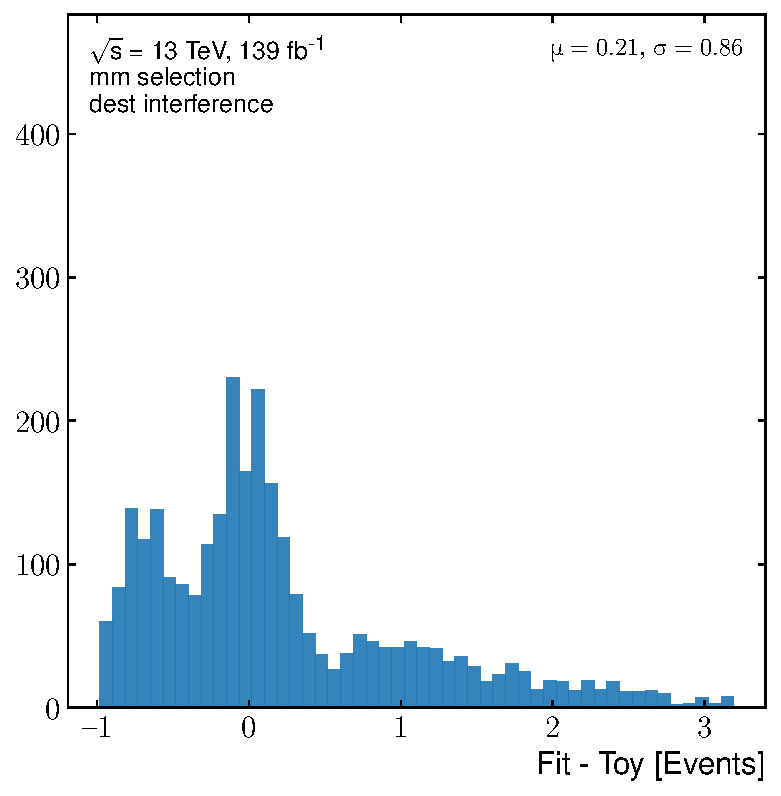
\includegraphics[width=\textwidth]{/Users/Deshan/Documents/PhD/thesis/Thesis/figures/analysis/bkgmodel/uncertainties/fitSs-mm-dest.pdf}
        \label{fig:bkgmodel:toyss4}
    \end{subfigure}
    \caption[Distributions of extrapolation from fit to poisson distributed toys generated in the control region]{Distribution of the difference between the expected background in the signal region from fits to poisson generated toys and the background estimation from the toy. The toys have been generated from the fit to the data in the control region. The mean and standard deviation of each distribution is also shown. The constructive (top) and destructive (bottom) signal regions for the electron (left) and muon (right) channels are shown.}
    \label{fig:bkgmodel:toyss}
\end{figure}

\subsubsection{Control region bias uncertainty}
The \emph{CR bias uncertainty}, \CRBU, on the expected background quantifies the residual difference between the two fit models, with and without the signal component, described in \cref{sec:modelchoice,sec:sigmodel}. Possible signals in data can result in the background estimate from the background-only fit model being biased. Whereas, the signal+background model is unaffected by the presence of signals. Using simulated samples, the difference between in two models is negligible by construction due to the optimisation of the CR choice. However, when fitting data, small differences between the two fit models can be present. The difference is taken as an additional uncertainty on the background estimate. The uncertainty attempts to quantify the degree to which signal-like shapes exist in data for a given CR choice. 

The \CRBU is measured by fitting both the background-only and signal+background fit models to data in the CR and extrapolating the background components of the two models to the SR. The background estimate is calculated by integrating the extrapolation in the SR. The difference between the resulting background estimates from the two fit models is used as the \CRBU. 

\subsection{Signal yield uncertainties}
The expected number of simulated CI signal events is used in the statistical analysis to produce results in terms of CI interaction models. The simulated contact interaction expected events in the SR are also affected by the theoretical and experimental uncertainties. The expected signal yield is obtained by integrating the simulated signal in the SR. An uncertainty is assigned to the expected yield by summing in quadrature the of the uncertainties associated with the signal yield. The theoretical and experimental uncertainties are treated separately and obtained from the procedure described in \cref{chap:sysmc}. Only the experimental uncertainties are used in the statistical analysis. Whereas, the theoretical uncertainties are quotes in the results section. 

\subsection{Summary of uncertainties}

The relative uncertainty on both the background estimate and expected signal yield is summarised in \cref{tab:summaryUncerts}. Due to the smaller size of the destructive signal regions, there is a smaller expected number of background events, which results in larger relative uncertainties in the SRs. The \CRBU has a minimal impact on the statistical analysis, and the most significant impact is from the \STATU.

\begin{table}[htp]
    \begin{center}
    \begingroup
    \setlength{\tabcolsep}{10pt} % Default value: 6pt
    \renewcommand{\arraystretch}{1.5} % Default value: 1
    {\small
    \begin{tabular}{l l | c c c | c c}
    \toprule
            &              & \multicolumn{3}{c|}{Background uncertainties} & \multicolumn{2}{c}{Signal uncertainties}\\
    Channel & Interference & \STATU & \ISSU & \CRBU & \EXPE & \THEO \\
    \hline
    \ee     & Constructive & 20\% & 4\%  & 2\% & 8\%                               & \footnotesize{$^{+11\%}_{-10\%}$}\\
    \ee     & Destructive  & 61\% & 8\% & 1\% & 8\%                               & \footnotesize{$^{+14\%}_{-13\%}$}\\
    $\mumu$ & Constructive & 21\% & 6\%  & 2\% & \footnotesize{$^{+20\%}_{-17\%}$} & \footnotesize{$^{+10\%}_{-9\%}$}\\
    $\mumu$ & Destructive  & 58\% & 24\% & 4\% & \footnotesize{$^{+27\%}_{-22\%}$} & \footnotesize{$^{+13\%}_{-12\%}$}\\
    \bottomrule
    \end{tabular}
    }
    \endgroup
    \label{tab:summaryUncerts}
    \end{center}
    \caption[Summary of the relative uncertainties on the background estimate and signal yield in each signal region]{Summary of the relative uncertainties on the background estimate and signal in each signal region, where \STATU is the ``statistical uncertainty of the fit'', \ISSU is the ``induced spurious signal uncertainty'' and \CRBU is the ``control region bias uncertainty''. Experimental and theoretical uncertainties are shown as well with the latter averaged across CI chirality scenarios and quoted for $\Lambda=30$~TeV only.}
\end{table}
